%! TEX root = task1_report.tex
\documentclass[11pt,a4paper]{article}

% ====================================================================
% Packages & Layout Configuration
% ====================================================================
\usepackage[utf8]{inputenc}
\usepackage[margin=0.85in]{geometry}
\usepackage{graphicx}
\usepackage{booktabs}
\usepackage{tabularx}
\usepackage{hyperref}
\usepackage{xurl}
\usepackage{listings}
\usepackage{xcolor}
\usepackage{titlesec}
\usepackage{fancyhdr}
\usepackage{float}
\usepackage{caption}
\usepackage{subcaption}
% Keep \texttt unbroken and push whole token to the next line if it does not fit
\let\oldtexttt\texttt
\renewcommand{\texttt}[1]{\mbox{\oldtexttt{#1}}}
\sloppy

% Set graphicspath to local screenshots folder
\graphicspath{{./screenshots/}}

% Hyperlink styling
\hypersetup{
    colorlinks=true,
    linkcolor=blue!75!black,
    citecolor=blue!75!black,
    urlcolor=blue!75!black
}

% Code listing styling
\definecolor{codegray}{rgb}{0.5,0.5,0.5}
\definecolor{codebackground}{rgb}{0.96,0.96,0.96}
\definecolor{codekeyword}{rgb}{0.13,0.13,1}
\definecolor{codestring}{rgb}{0.63,0.13,0.94}

\lstdefinestyle{customcode}{
    backgroundcolor=\color{codebackground},
    basicstyle=\ttfamily\footnotesize,
    breaklines=true,
    captionpos=b,
    commentstyle=\color{codegray},
    keywordstyle=\color{codekeyword}\bfseries,
    stringstyle=\color{codestring},
    frame=single,
    tabsize=2,
    showstringspaces=false
}
\lstset{style=customcode}

% Page header & footer
\pagestyle{fancy}
\fancyhf{}
\lhead{\textbf{SWE40006 Software Deployment and Evolution}}
\cfoot{\thepage}

\begin{document}

% ====================================================================
% Mandated Header (Student details, Unit details, Dates, Task level)
% ====================================================================
\begin{center}
    {\LARGE \textbf{Deployment Portfolio Task 1}}\\[0.2cm]
    {\large \textit{Desktop deployment using the Windows Installer XML (WiX) tool}}\\[0.1cm]
\end{center}

\noindent\rule{\textwidth}{1pt}\par\vspace{0.2cm}
\begin{enumerate}
    \item \textbf{Student details:}
    \begin{itemize}
        \item \textbf{Student ID:} 105559691
        \item \textbf{Full name:} Dang Duc Minh
    \end{itemize}
    \item \textbf{Unit details:}
    \begin{itemize}
        \item \textbf{Unit code and Name:} SWE40006 Software Deployment and Evolution
        \item \textbf{Semester:} Semester 3, 2026
    \end{itemize}
    \item \textbf{Due date and submission date:}
    \begin{itemize}
        \item \textbf{Due date:} 28 September 2026, 23:59
        \item \textbf{Submission date:} 28 September 2026
    \end{itemize}
    \item \textbf{Declaration of the task level attempted:}
    \begin{itemize}
        \item \textbf{Level Attempted:} High Distinction (Sub-tasks 1.1 to 1.4)
        \item \textbf{Source code:}
        \begin{itemize}
            \item \textbf{Task 1.1 (SampleApp):} \url{https://github.com/mikedevman/SWE40006/tree/master/task1/task1.1/SampleApp}
            \item \textbf{Tasks 1.2 to 1.4 (AlphtechDSP 2.0):} \url{https://github.com/mikedevman/AlphtechDSP-2.0}
        \end{itemize}
    \end{itemize}
\end{enumerate}
\noindent\rule{\textwidth}{1pt}

\newpage

% ====================================================================
% Task 1.1: Baseline Desktop Deployment (Pass Tier)
% ====================================================================
\section*{Task 1.1 (Pass):}

\begin{figure}[H]
    \centering
    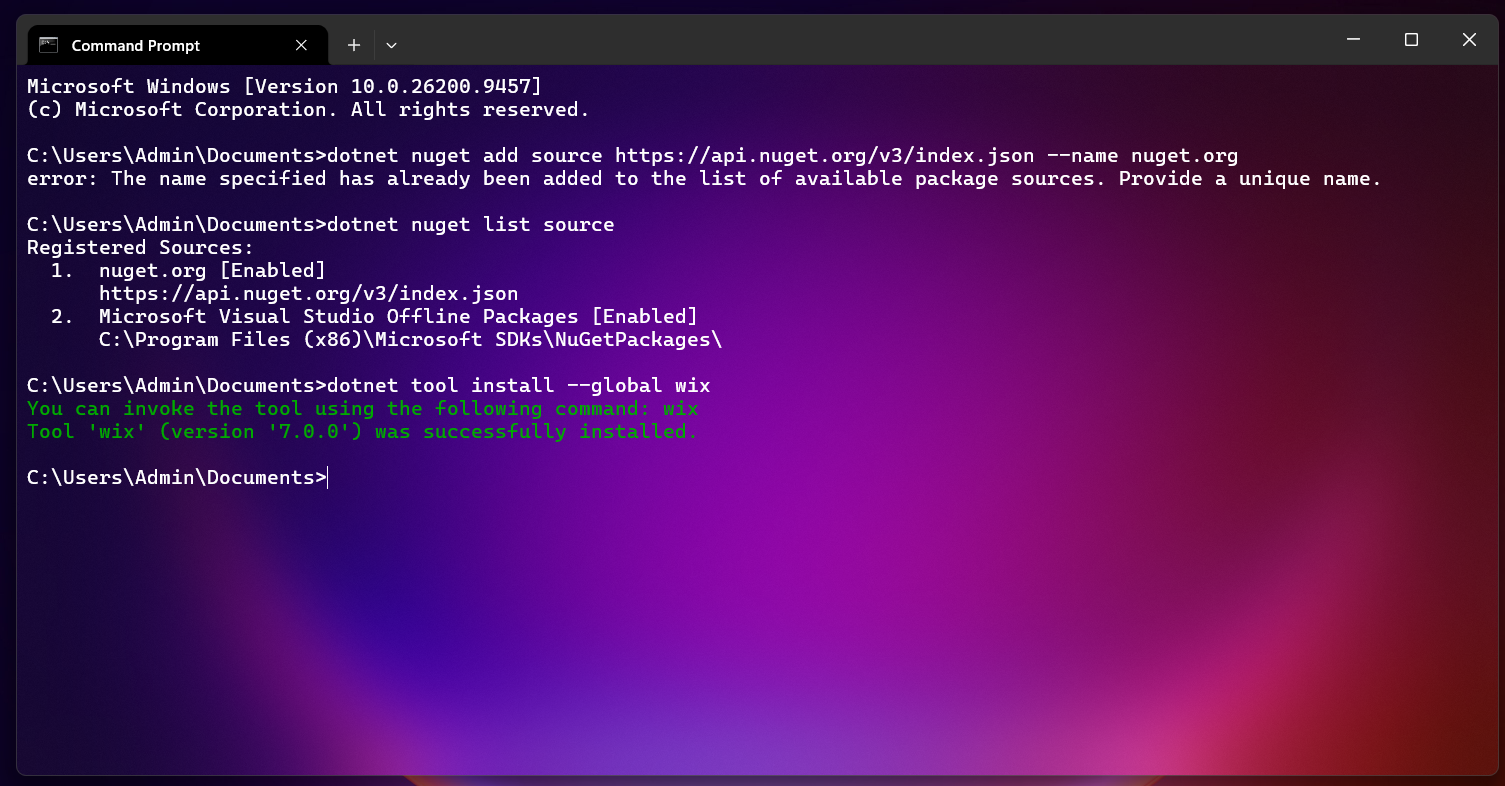
\includegraphics[width=0.80\linewidth]{1.1_0.png}
    \caption{Installing the WiX toolset globally via the CLI.}
\end{figure}

\noindent To get started, the development environment needed to be set up for WiX. Using the CLI, the NuGet package source was checked and the WiX toolset was installed globally with \texttt{dotnet tool install --global wix}, which pulled in version 7.0.0.

\begin{figure}[H]
    \centering
    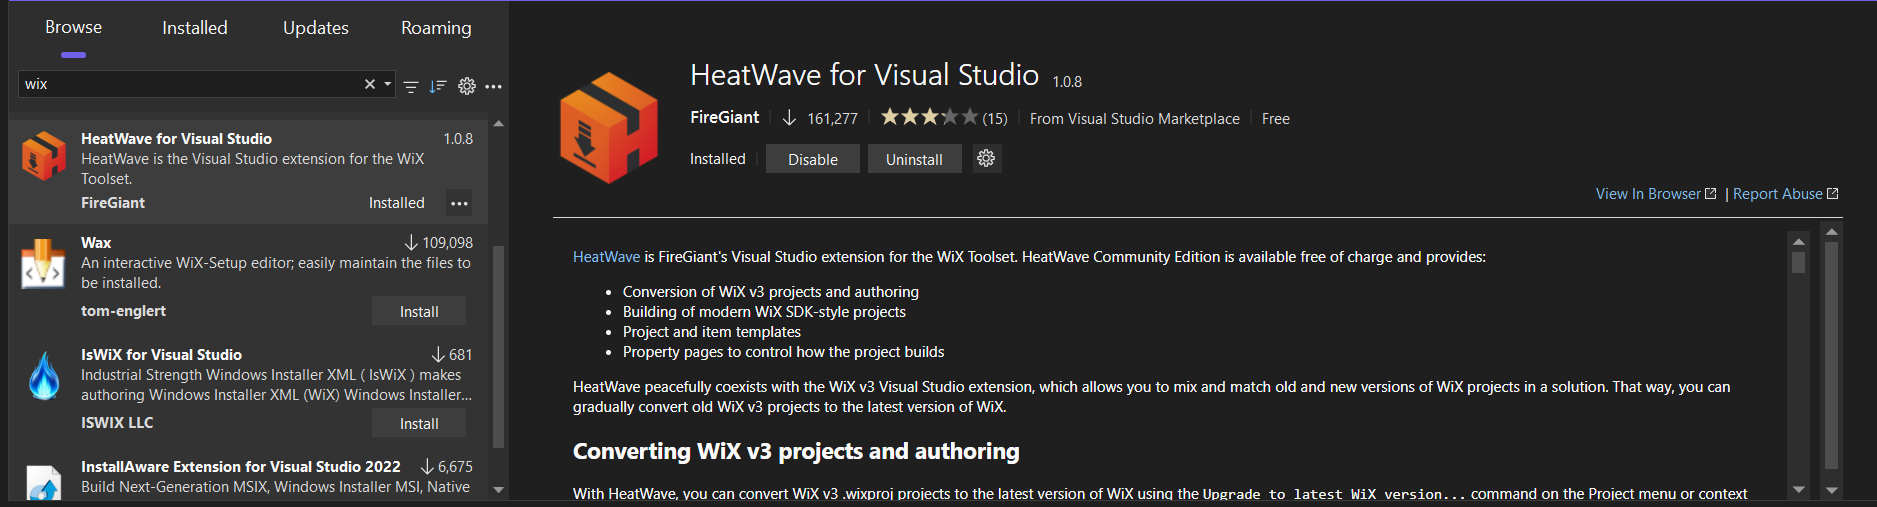
\includegraphics[width=0.60\linewidth]{1.1_1.png}
    \caption{HeatWave for Visual Studio extension installed and enabled.}
\end{figure}

\noindent The next thing was to set up WiX on Visual Studio. The \textbf{HeatWave for Visual Studio} extension by FireGiant was installed from the Visual Studio Marketplace. This adds WiX project templates and build support directly to the Visual Studio IDE.

\vspace{100pt}

\begin{figure}[H]
    \centering
    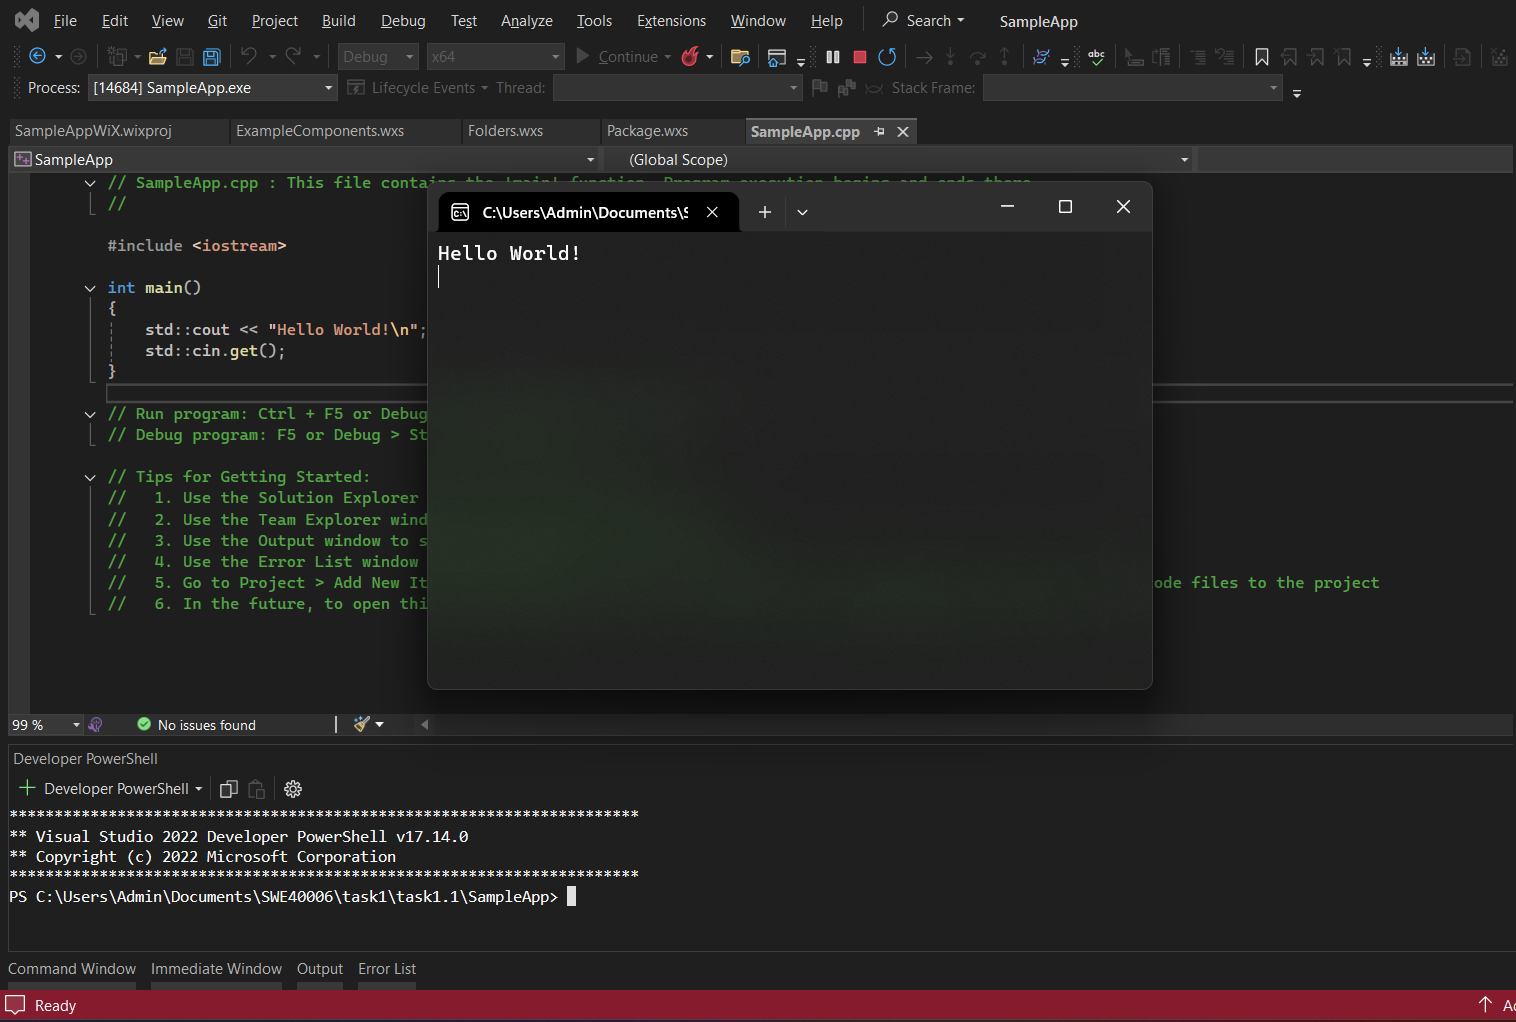
\includegraphics[width=0.60\linewidth]{1.1_2.png}
    \caption{SampleApp compiled and running successfully in Visual Studio 2022.}
\end{figure}

\noindent The sample application, \texttt{SampleApp}, is a simple C++ console program that prints ``Hello World!'' (can be found in this GitHub repository: \url{https://github.com/mikedevman/SWE40006/tree/master/task1/task1.1/SampleApp}). The project was built and run to make sure everything works before packaging it.

\begin{figure}[H]
    \centering
    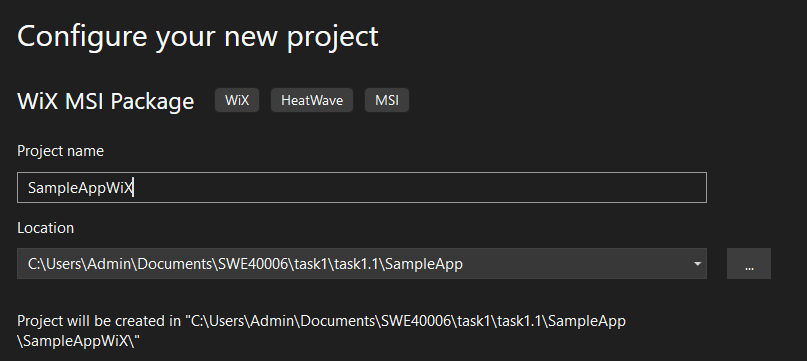
\includegraphics[width=0.60\linewidth]{1.1_3.png}
    \caption{Configuring the new WiX MSI Package project named SampleAppWiX.}
\end{figure}

\noindent To create the installer project, a new \textbf{WiX MSI Package} project was added to the solution via HeatWave. The project was named \texttt{SampleAppWiX} and placed inside the existing \texttt{SampleApp} solution directory so that both projects live under the same solution.

\begin{figure}[H]
    \centering
    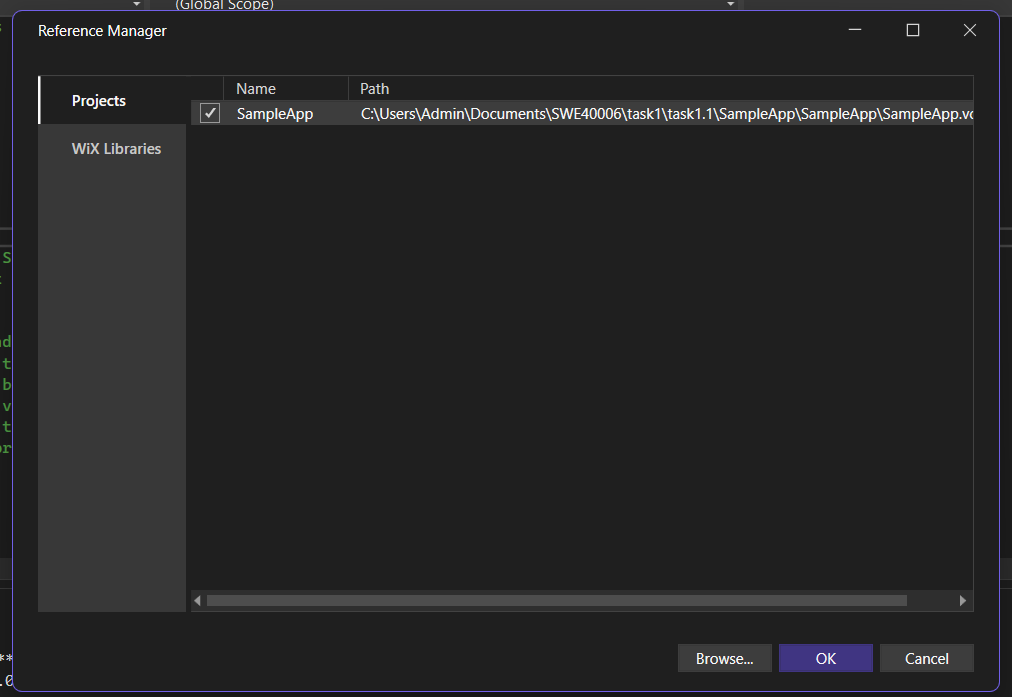
\includegraphics[width=0.60\linewidth]{1.1_4.png}
    \caption{Adding a project reference from SampleAppWiX to SampleApp.}
\end{figure}

\noindent A project reference was then added from \texttt{SampleAppWiX} to \texttt{SampleApp} through the Reference Manager. This link lets the WiX build process automatically find the compiled \texttt{SampleApp.exe}, so the installer always packages the latest build.

\begin{figure}[H]
    \centering
    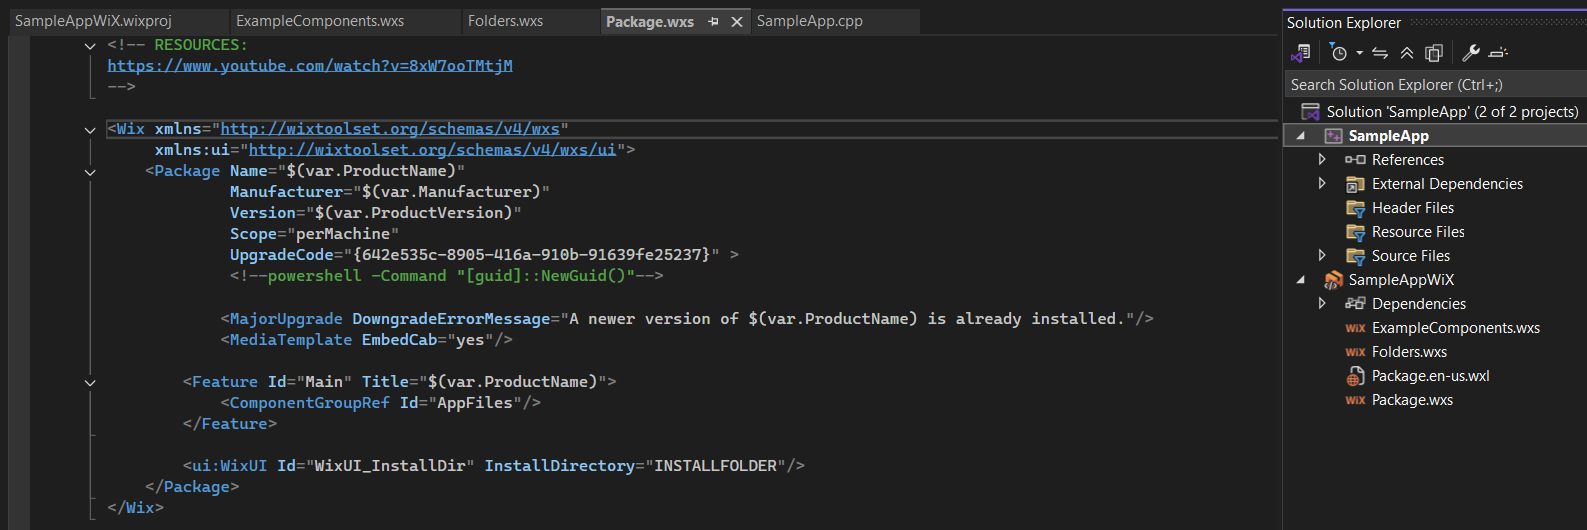
\includegraphics[width=0.60\linewidth]{1.1_5.png}
    \caption{The authored \texttt{Package.wxs} manifest.}
\end{figure}

\noindent The main installer configuration lives in \texttt{Package.wxs}. This file sets the product name, an upgrade code for version management, per-machine scope attribute, a \texttt{MajorUpgrade} element to block downgrades, and a \texttt{MediaTemplate} to embed the cabinet files (compressed archives holding the application binaries). A \texttt{Feature} element groups the app files, and a \texttt{WixUI} reference adds the standard setup wizard dialogs.

\noindent \texttt{ExampleComponent.wxs} and \texttt{Folders.wxs} files were also configured to define the installation folder inside Program Files and specify the executable file to deploy along with its shortcuts.

\vspace{100pt}

\begin{figure}[H]
    \centering
    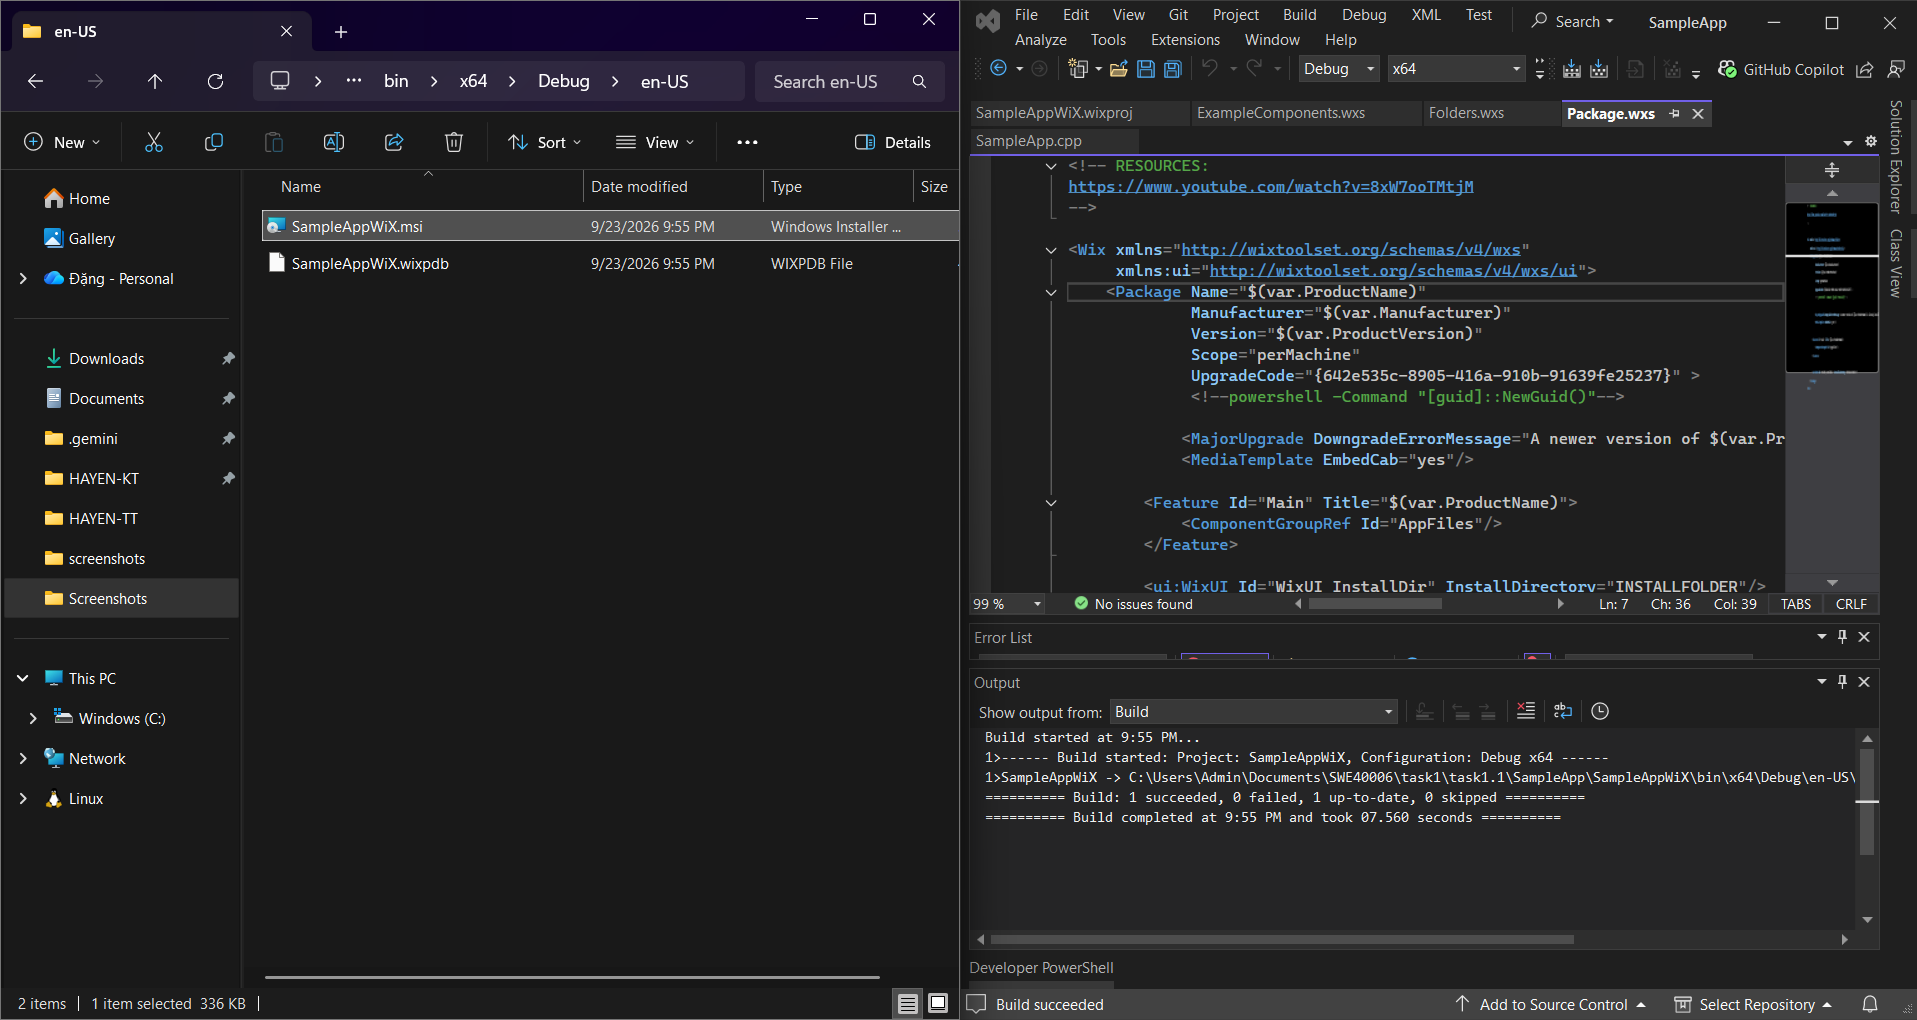
\includegraphics[width=0.60\linewidth]{1.1_6.png}
    \caption{Successful build producing \texttt{SampleAppWiX.msi} in the output directory.}
\end{figure}

\noindent Building the \texttt{SampleAppWiX} project created the final \texttt{SampleAppWiX.msi} installer in the output folder.

\begin{figure}[H]
    \centering
    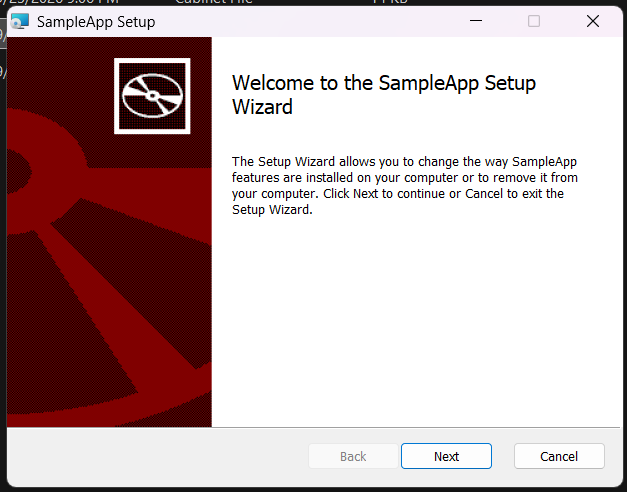
\includegraphics[width=0.60\linewidth]{1.1_7.png}
    \caption{The SampleApp Setup Wizard.}
\end{figure}

\noindent Double-clicking the MSI file opened the Windows Installer setup wizard. The dialog shows the product name and gives users options for program installation configuration.

\vspace{100pt}

\begin{figure}[H]
    \centering
    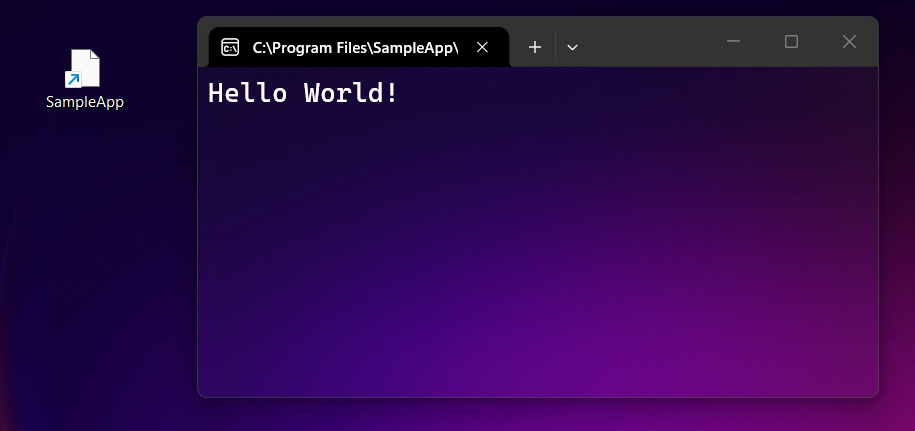
\includegraphics[width=0.60\linewidth]{1.1_8.png}
    \caption{SampleApp running from the installed Program Files directory.}
\end{figure}

\noindent After finishing the installation, the application was placed in \texttt{C:\textbackslash Program Files\textbackslash SampleApp}. Opening the executable file showed the console prints ``Hello World!'' and the application shortcut is visible on the desktop.

% ====================================================================
% Task 1.2: Custom Desktop Deployment (Credit Tier)
% ====================================================================
\section*{Task 1.2 (Credit):}

\begin{figure}[H]
    \centering
    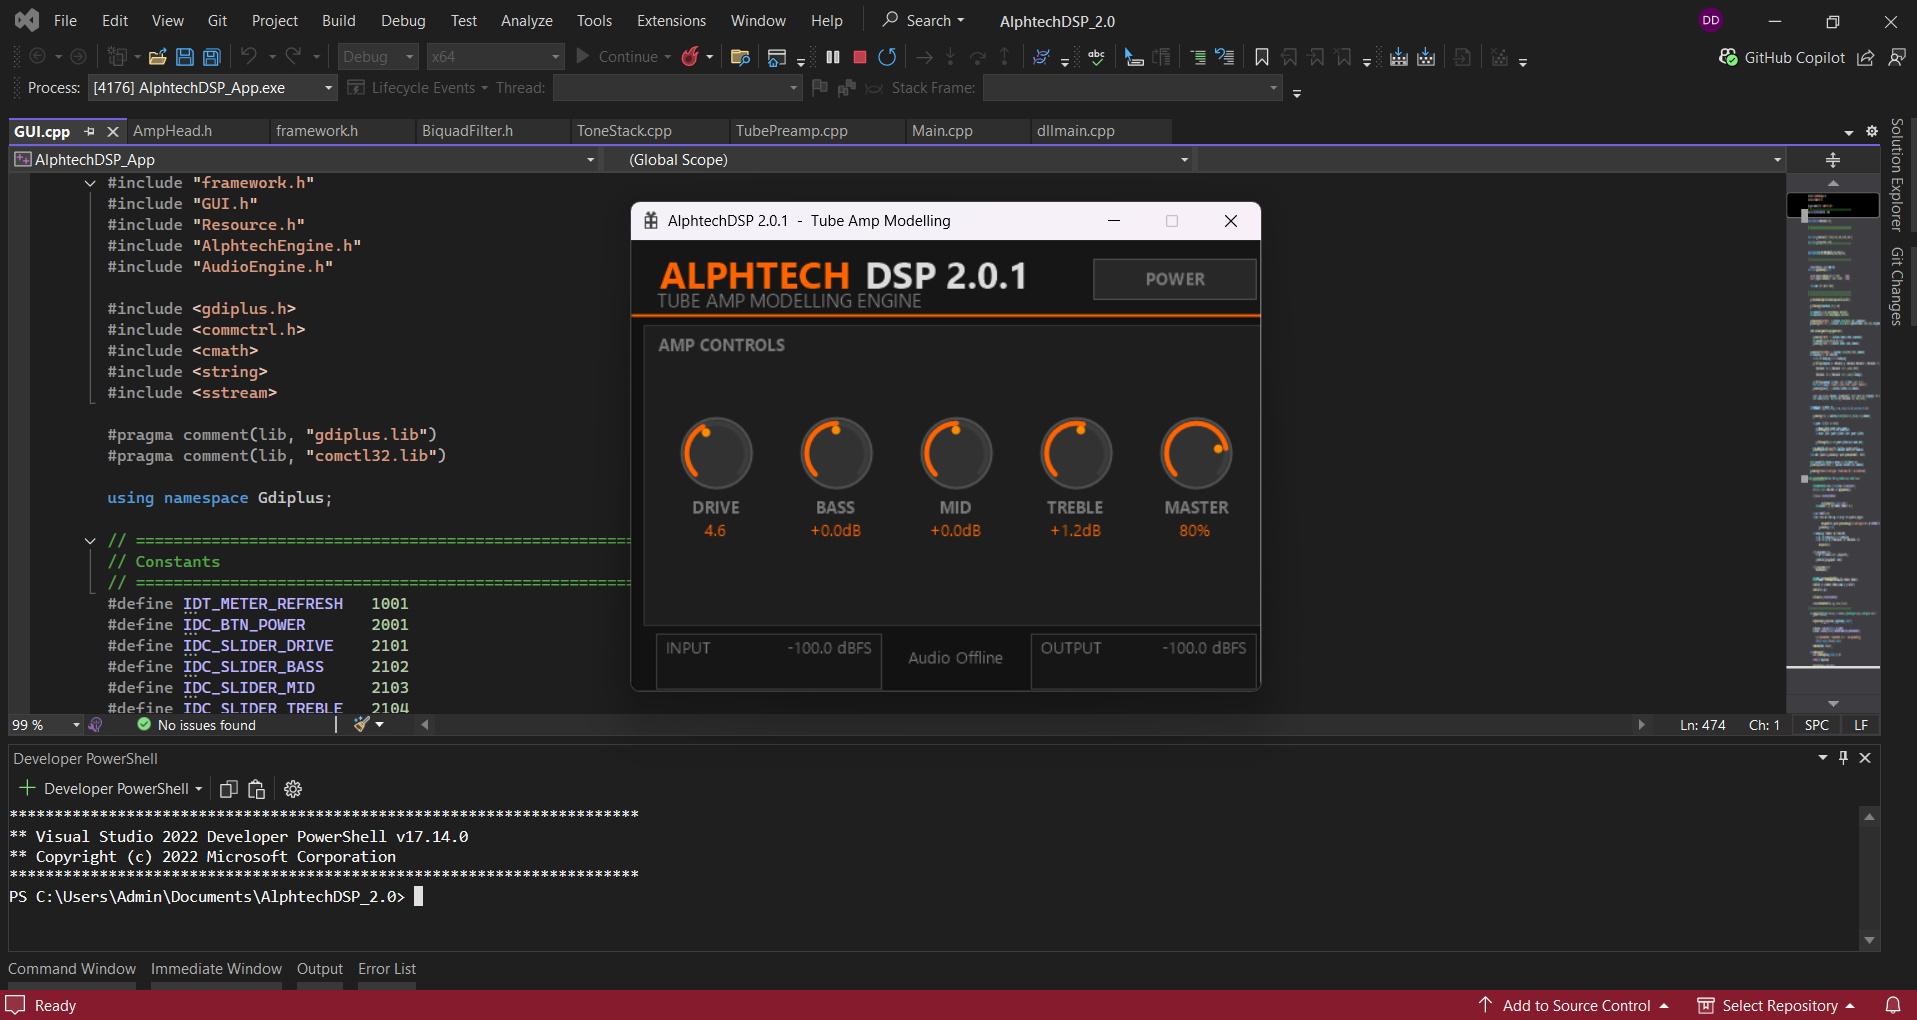
\includegraphics[width=0.60\linewidth]{1.2_1.png}
    \caption{AlphtechDSP 2.0 running in Visual Studio 2022.}
\end{figure}

\noindent With the basic WiX workflow done in Task 1.1, the next step was to apply the same process to a custom application. The target here is \textbf{AlphtechDSP 2.0}, my personal C++ project that models a virtual guitar preamp (can be found in this GitHub repository: \url{https://github.com/mikedevman/AlphtechDSP-2.0}). It includes real-time audio I/O Digital Signal Processing (DSP), with adjustable drive gain and a 3-band EQ. The application was built and run to make sure everything works before packaging.

\vspace{100pt}

\begin{figure}[H]
    \centering
    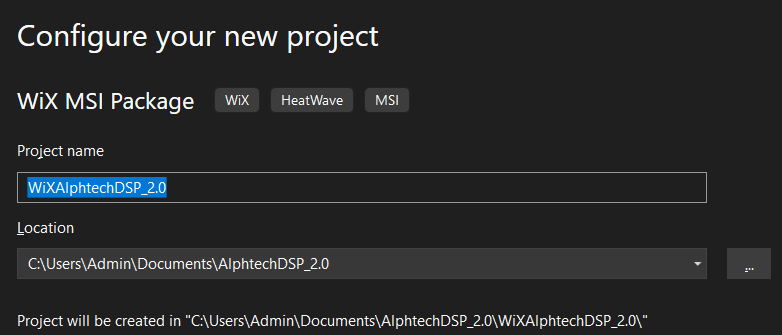
\includegraphics[width=0.60\linewidth]{1.2_2.png}
    \caption{Configuring the new WiX MSI Package project named WiXAlphtechDSP\_2.0.}
\end{figure}

\noindent A new \textbf{WiX MSI Package} project was added to the AlphtechDSP solution using the same HeatWave template from Task 1.1. The installer project was named \texttt{WiXAlphtechDSP\_2.0} and placed inside the existing solution directory.

\begin{figure}[H]
    \centering
    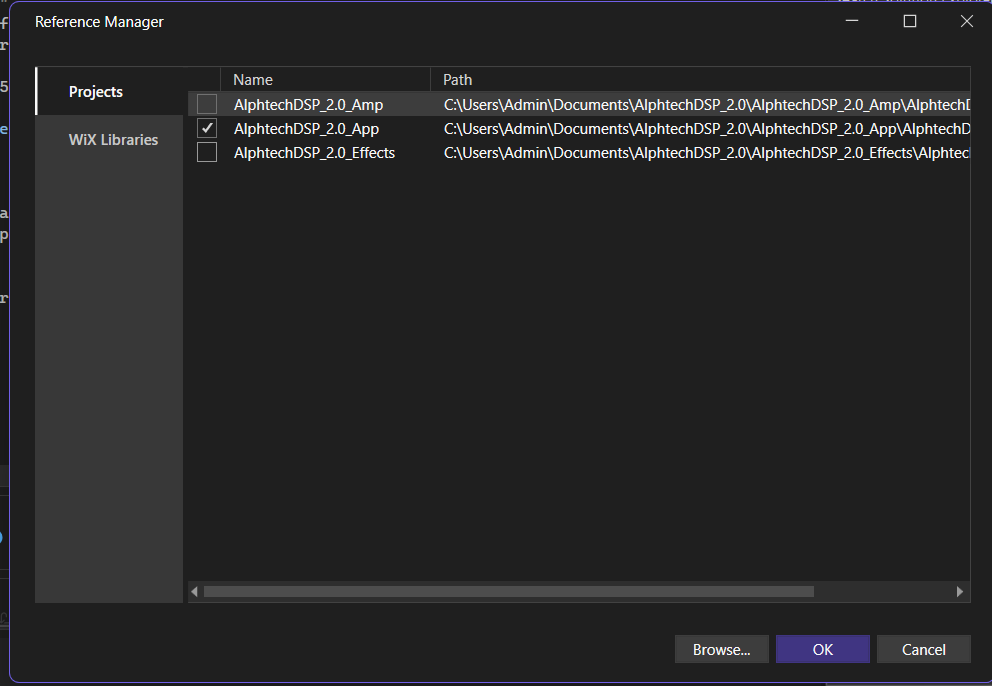
\includegraphics[width=0.60\linewidth]{1.2_3.png}
    \caption{Adding a project reference to AlphtechDSP\_2.0\_App only.}
\end{figure}

\noindent The Reference Manager was opened to link the installer to the application. The solution has three projects: \texttt{AlphtechDSP\_2.0\_Amp}, \texttt{AlphtechDSP\_2.0\_Effects}, and \texttt{AlphtechDSP\_2.0\_App}. For this initial deployment, only the main application project \texttt{AlphtechDSP\_2.0\_App} was selected. The two DLL projects were left unchecked on purpose to show what happens when dependencies are missing.

\vspace{100pt}

\begin{figure}[H]
    \centering
    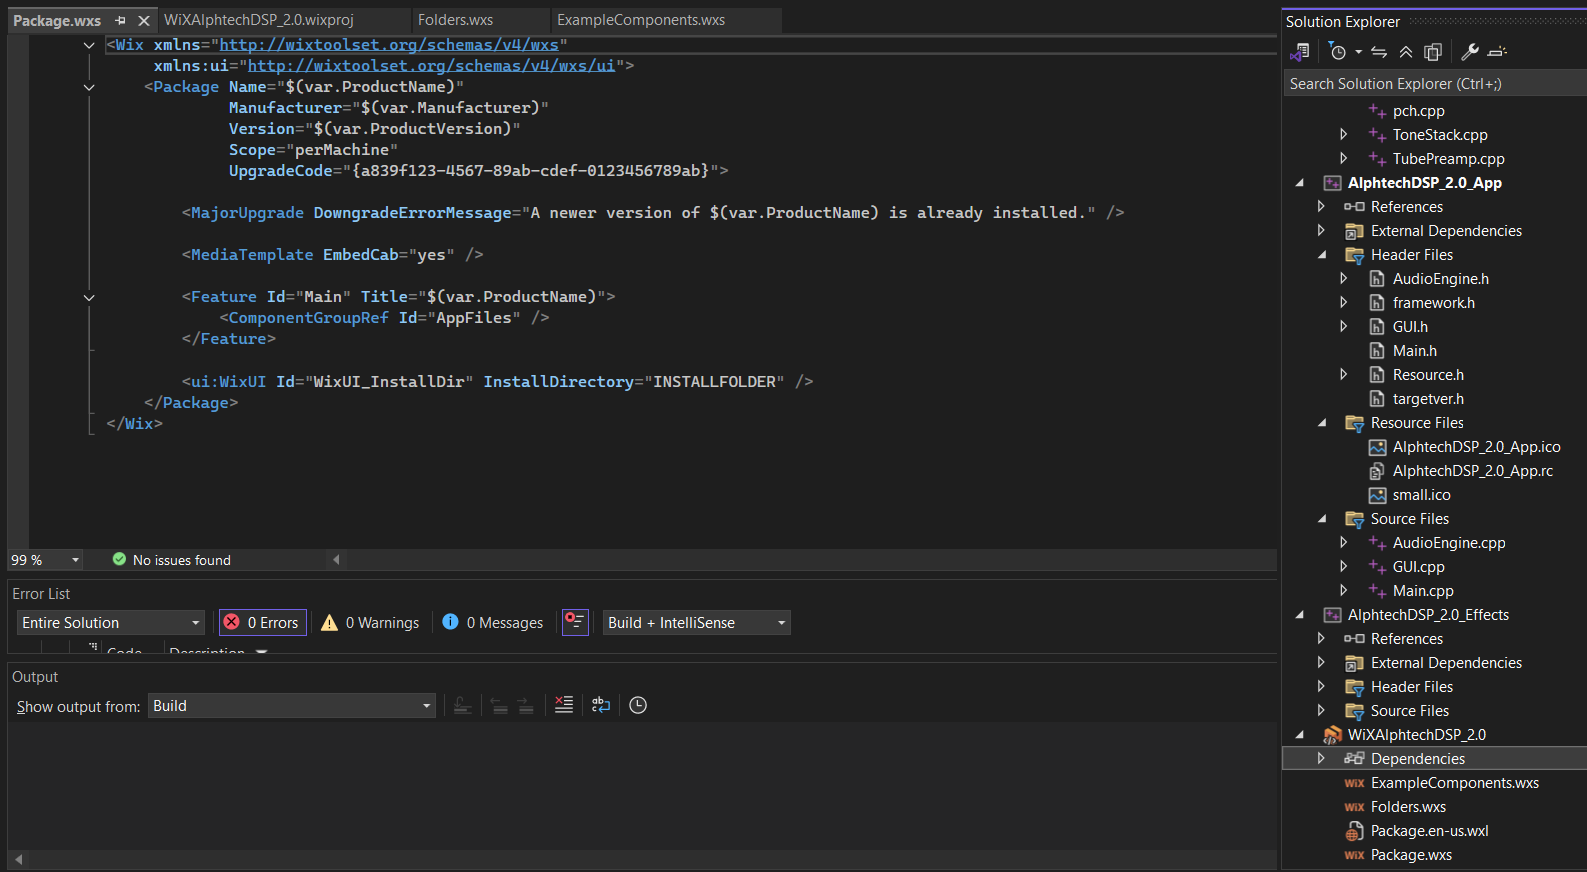
\includegraphics[width=0.60\linewidth]{1.2_4.png}
    \caption{The authored Package.wxs manifest.}
\end{figure}

\noindent The WiX manifest files were then written. \texttt{Package.wxs} was set up with the product name, manufacturer, version, and an upgrade code. The \texttt{WixUI\_InstallDir} dialog set was included to give the user a full setup wizard with folder selection. The \texttt{Folders.wxs} and \texttt{ExampleComponents.wxs} files were also configured alongside it.

\begin{figure}[H]
    \centering
    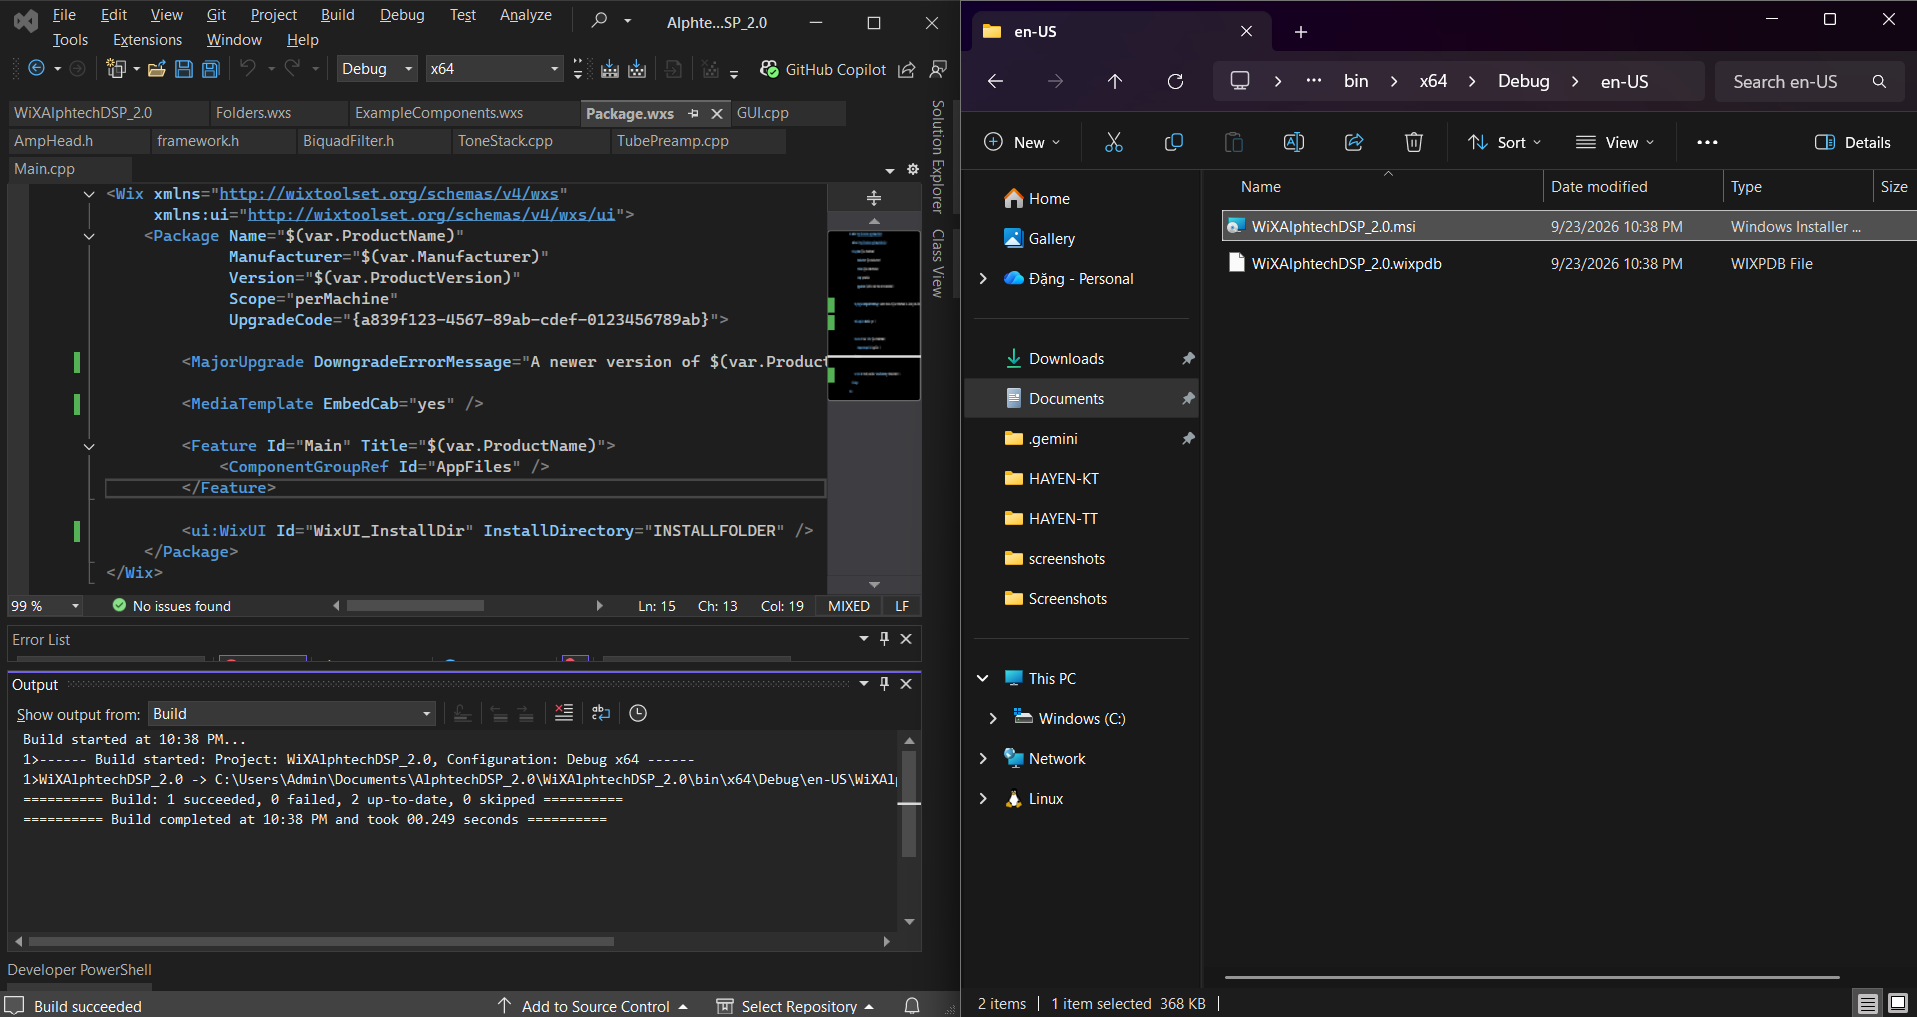
\includegraphics[width=0.60\linewidth]{1.2_5.png}
    \caption{Successful build producing WiXAlphtechDSP\_2.0.msi in the output directory.}
\end{figure}

\noindent Building the installer project created \texttt{WiXAlphtechDSP\_2.0.msi} in the output folder. The output terminal showed a clean build with 1 succeeded and 0 failed.

\begin{figure}[H]
    \centering
    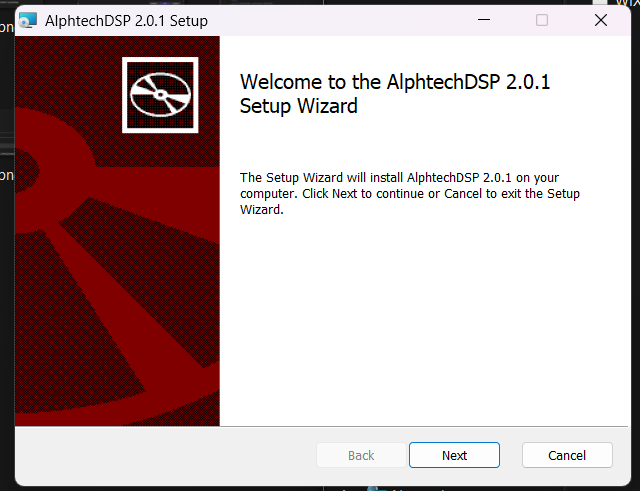
\includegraphics[width=0.60\linewidth]{1.2_6.png}
    \caption{The AlphtechDSP 2.0.1 Setup Wizard launched from the generated MSI.}
\end{figure}

\noindent Running the MSI opened the AlphtechDSP 2.0.1 Setup Wizard, showing that the installer metadata were set up correctly.

\begin{figure}[H]
    \centering
    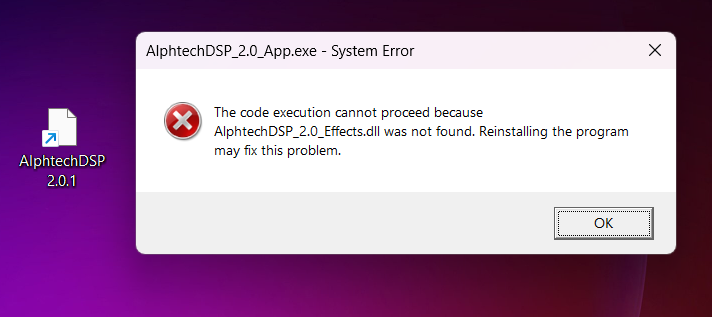
\includegraphics[width=0.55\linewidth]{1.2_7.png}
    \caption{System error: AlphtechDSP\_2.0\_Effects.dll was not found.}
\end{figure}

\begin{figure}[H]
    \centering
    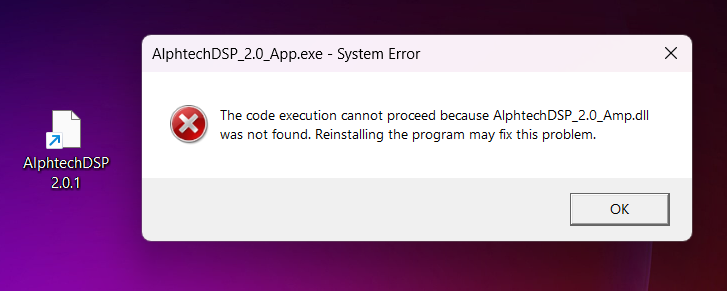
\includegraphics[width=0.55\linewidth]{1.2_8.png}
    \caption{System error: AlphtechDSP\_2.0\_Amp.dll was not found.}
\end{figure}

\noindent After the installation finished and the application was launched from the desktop shortcut, a system error popped up right away. Windows said that \texttt{AlphtechDSP\_2.0\_Effects.dll} and \texttt{AlphtechDSP\_2.0\_Amp.dll} were not found, which stopped the application from starting. This happened because only the executable was packaged and the shared DLL files were not included in the installer.
This confirmed that the application needs both DLL files to run and this failure leads to Task 1.3, where both DLLs will be added to the installer.

% ====================================================================
% Task 1.3: Multi-Component & Dual DLL Deployment (Distinction Tier)
% ====================================================================
\section*{Task 1.3 (Distinction):}

\begin{figure}[H]
    \centering
    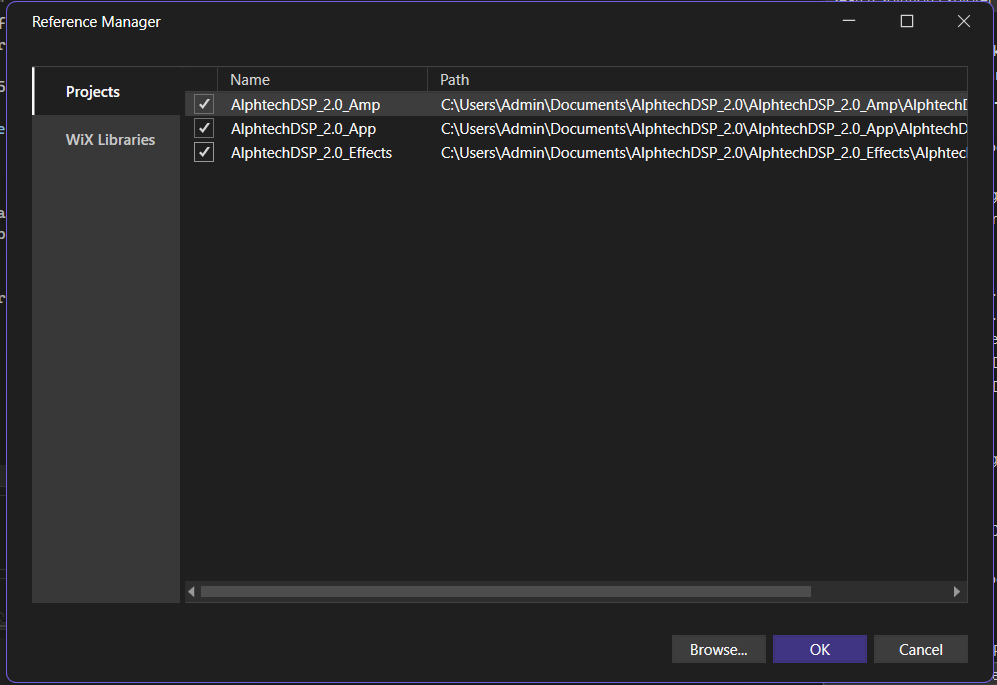
\includegraphics[width=0.65\linewidth]{1.3_1.png}
    \caption{All three project references now checked in the Reference Manager.}
\end{figure}

\noindent In order to fix the missing DLL files errors in Task 1.2, the installer needed to include all the runtime files. The first step was to go back to the Reference Manager and check all three projects: \texttt{AlphtechDSP\_2.0\_App}, \texttt{AlphtechDSP\_2.0\_Amp}, and \texttt{AlphtechDSP\_2.0\_Effects}, so the WiX installer can find every output binary.

\begin{figure}[H]
    \centering
    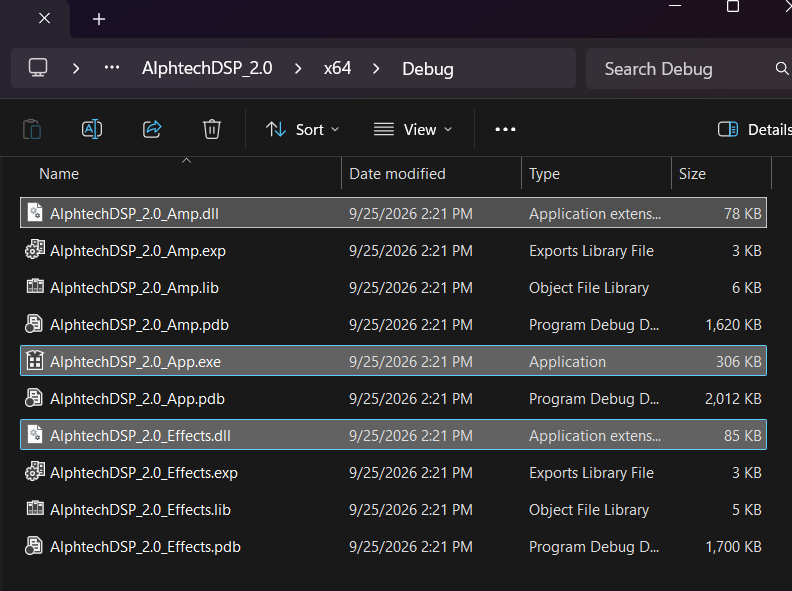
\includegraphics[width=0.60\linewidth]{1.3_2.png}
    \caption{Build output directory showing the executable and both DLLs.}
\end{figure}

\noindent The solution was rebuilt to generate the missing libraries. Both \texttt{AlphtechDSP\_2.0\_Amp.dll} and \texttt{AlphtechDSP\_2.0\_Effects.dll} had been produced next to \texttt{AlphtechDSP\_2.0\_App.exe} in the \texttt{x64\textbackslash Debug} output folder.

\begin{figure}[H]
    \centering
    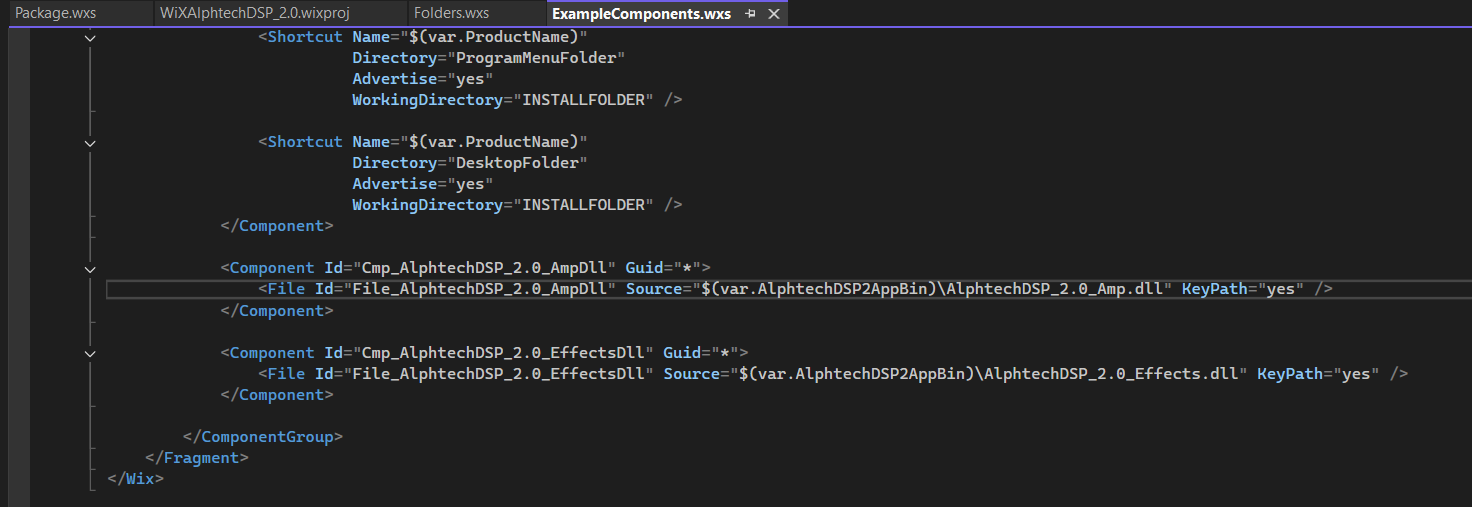
\includegraphics[width=0.60\linewidth]{1.3_3.png}
    \caption{Updated ExampleComponents.wxs with both DLL components declared.}
\end{figure}

\noindent The \texttt{ExampleComponents.wxs} manifest was then updated to add a separate \texttt{Component} for each DLL. Below the main executable component, two new components (\texttt{AlphtechDSP\_2.0\_Amp.dll} and \texttt{AlphtechDSP\_2.0\_Effects.dll}) were added. Both go into the same \texttt{INSTALLFOLDER} as the executable so Windows can find them when the app starts.

\begin{figure}[H]
    \centering
    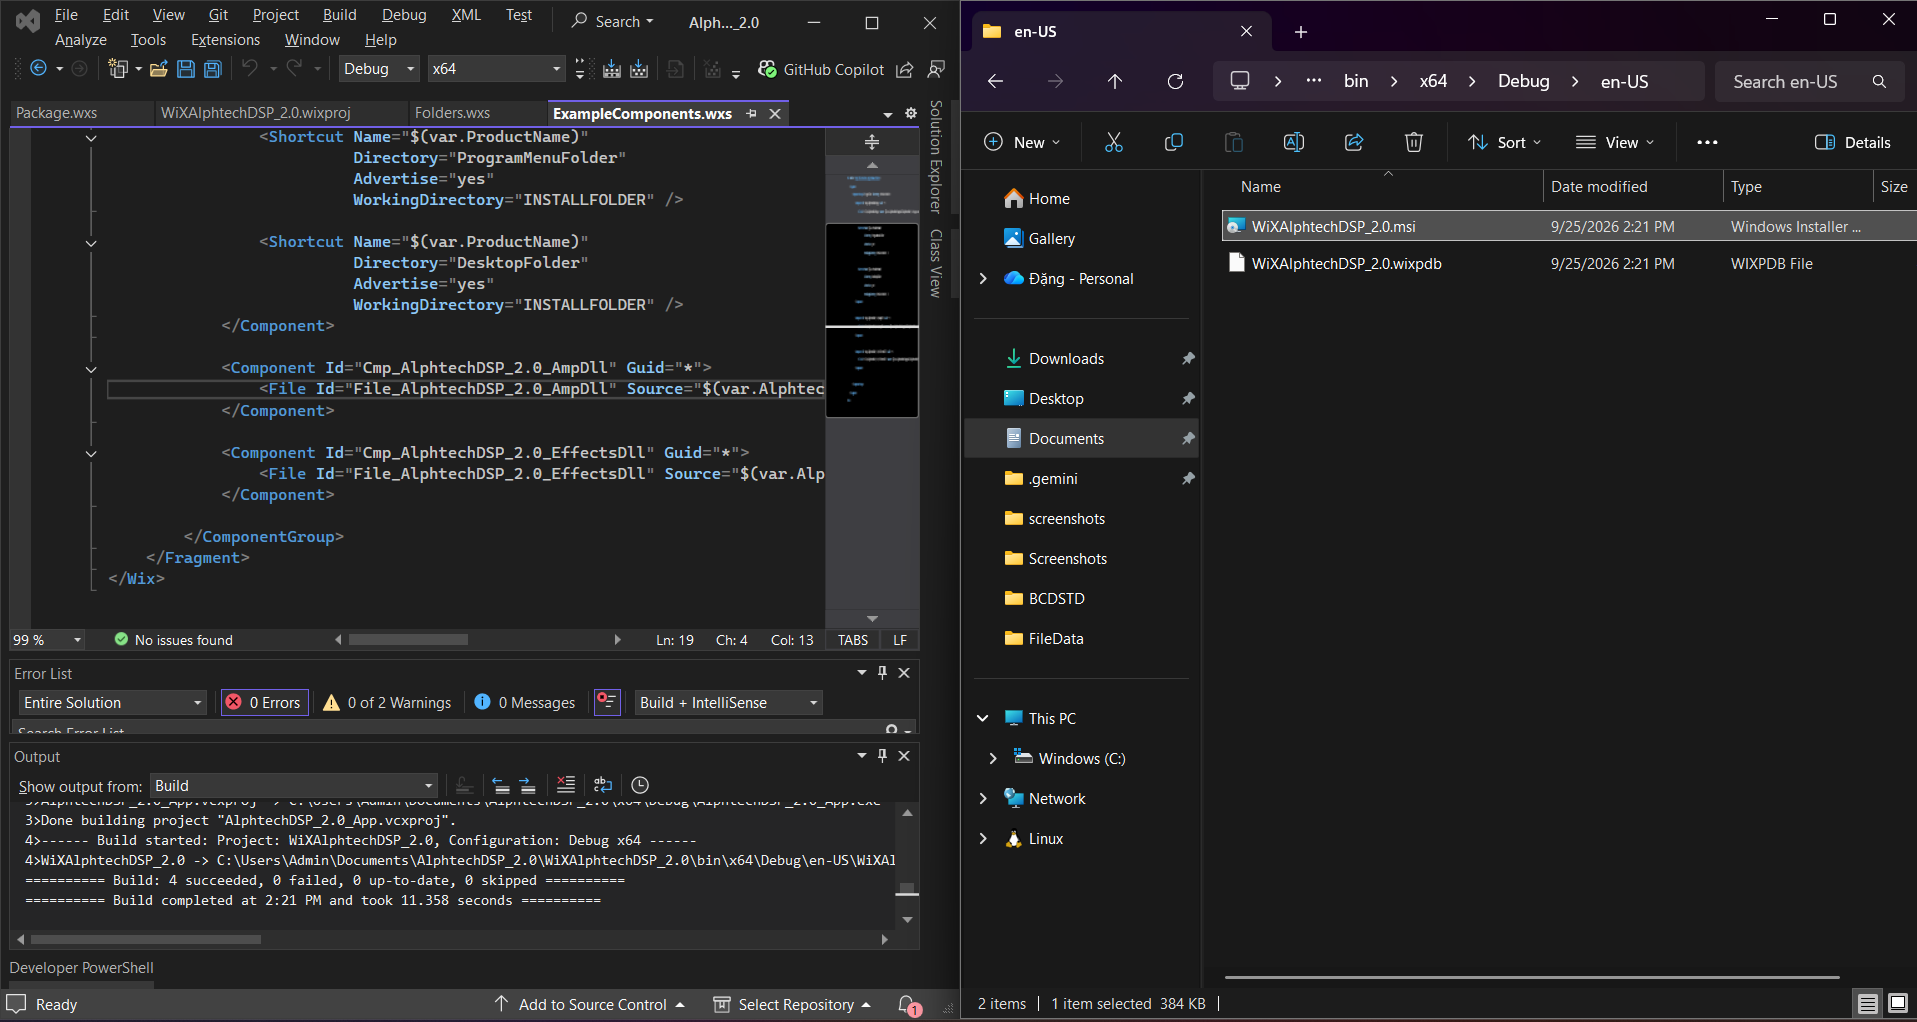
\includegraphics[width=0.60\linewidth]{1.3_4.png}
    \caption{Successful build of all four projects and the updated MSI in File Explorer.}
\end{figure}

\noindent Rebuilding the solution now compiled all four projects: the three application projects and the WiX installer. The output terminal showed 4 succeeded and 0 failed, and the updated \texttt{WiXAlphtechDSP\_2.0.msi} appeared in the output folder.

\begin{figure}[H]
    \centering
    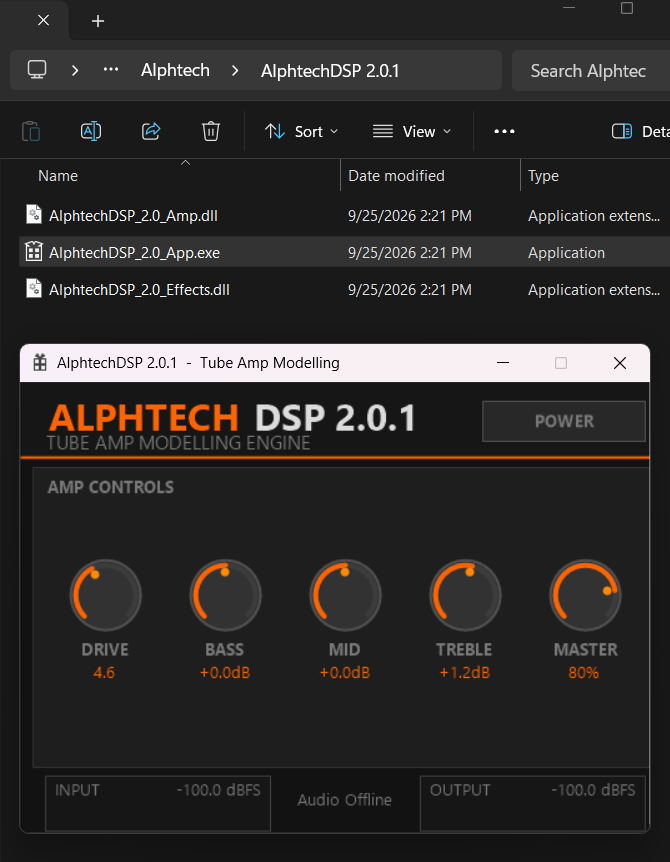
\includegraphics[width=0.60\linewidth]{1.3_5.png}
    \caption{AlphtechDSP 2.0 ran successfully with all dependencies resolved.}
\end{figure}

\noindent After running the updated installer, the folder at \texttt{Program Files\textbackslash Alphtech\textbackslash AlphtechDSP 2.0.1} now has all three files: the executable and both DLLs sitting together. Launching the application opened the AlphtechDSP 2.0 interface immediately without any missing DLL errors, which confirms that including the DLLs in the installer fixed the issues from Task 1.2.

% ====================================================================
% Task 1.4: Universal Windows App Packaging & Store Deployment (High Distinction Tier)
% ====================================================================
\section*{Task 1.4 (High Distinction):}

\begin{figure}[H]
    \centering
    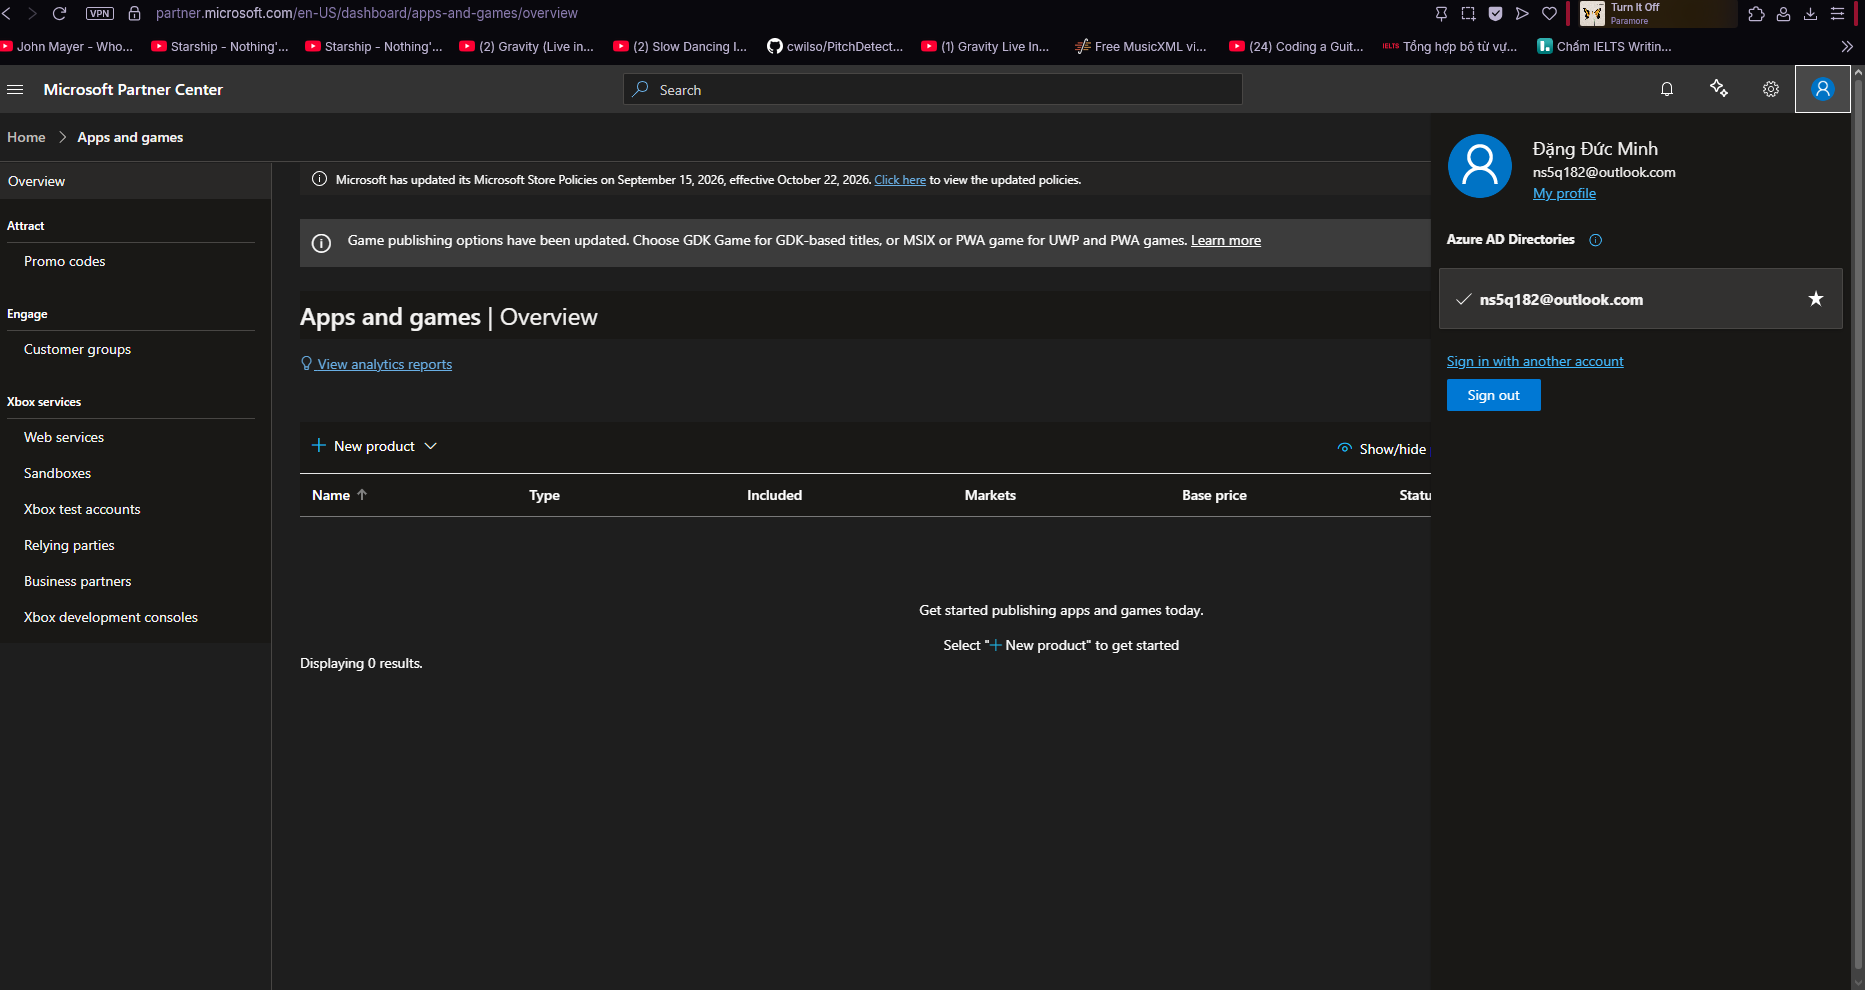
\includegraphics[width=0.60\linewidth]{1.4_0.png}
    \caption{Logging into Microsoft Partner Center and setting up a developer profile.}
\end{figure}

\noindent I started this task by logging into the Microsoft Partner Center and setting up my developer profile.

\begin{figure}[H]
    \centering
    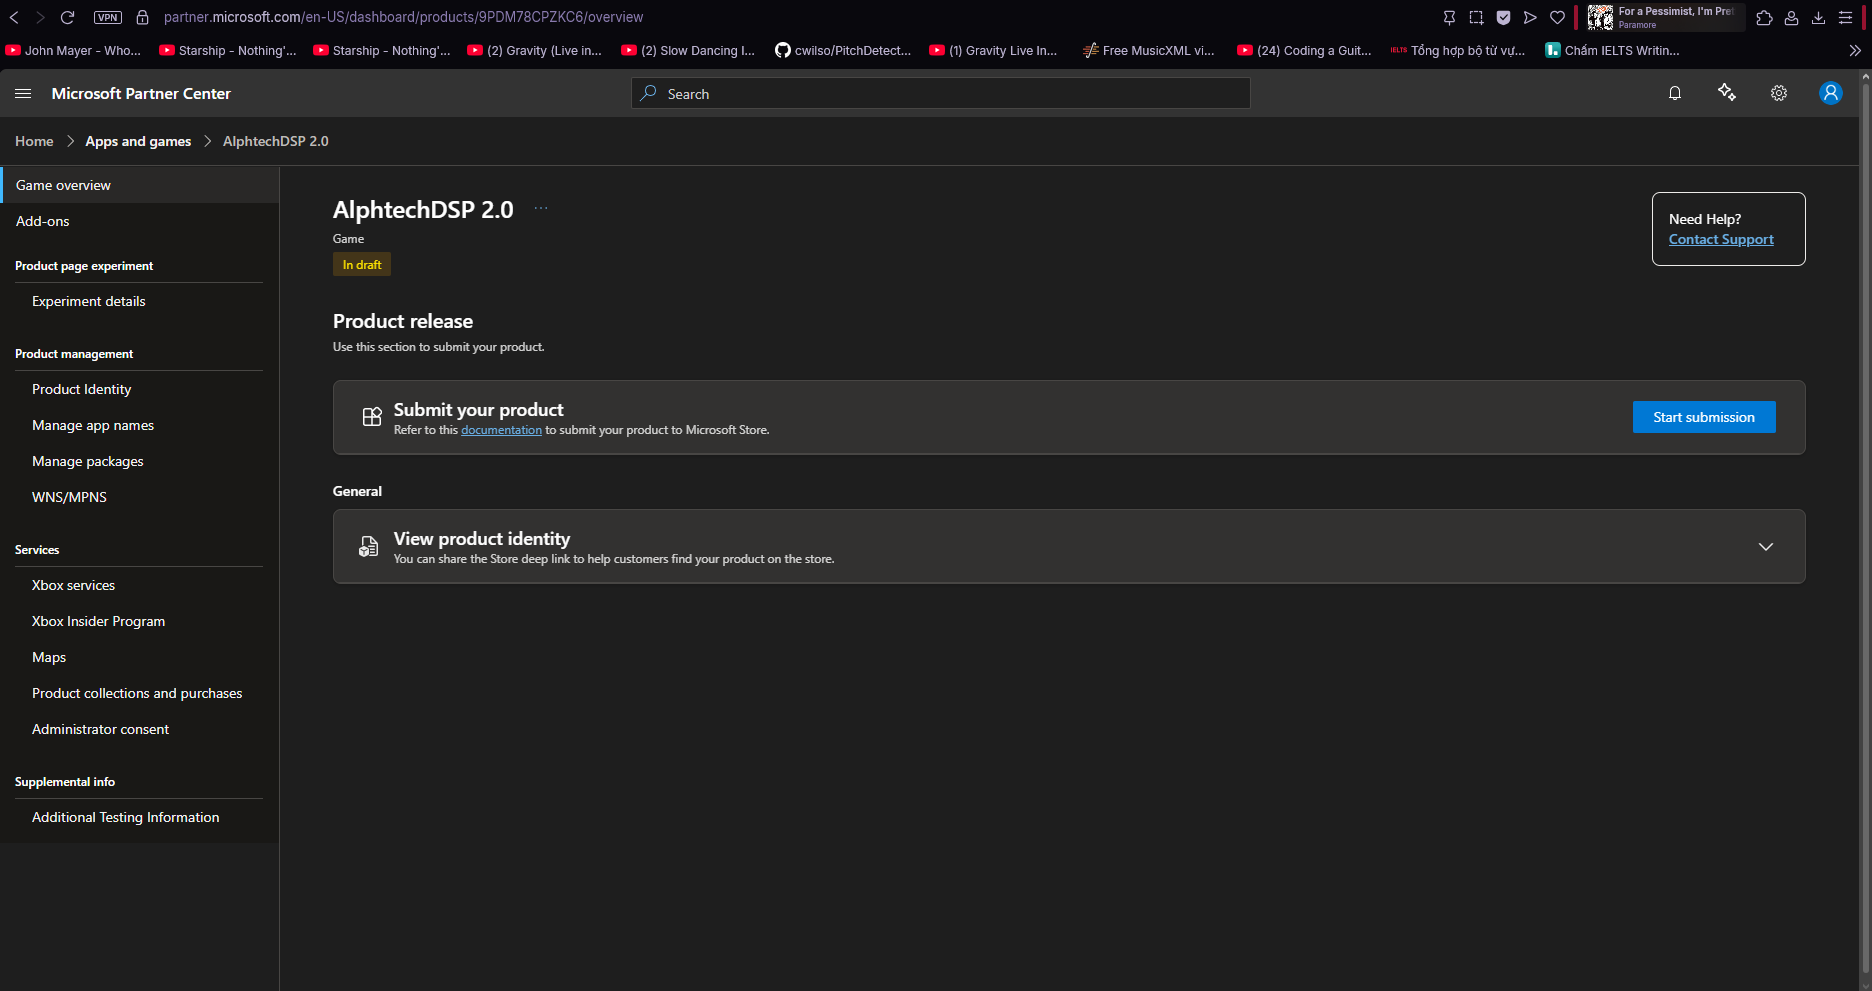
\includegraphics[width=0.60\linewidth]{1.4_0.5.png}
    \caption{Reserving the app name AlphtechDSP 2.0.}
\end{figure}

\noindent Once my profile was ready, I created a new app submission and reserved the name \textbf{AlphtechDSP 2.0} for the project.

\begin{figure}[H]
    \centering
    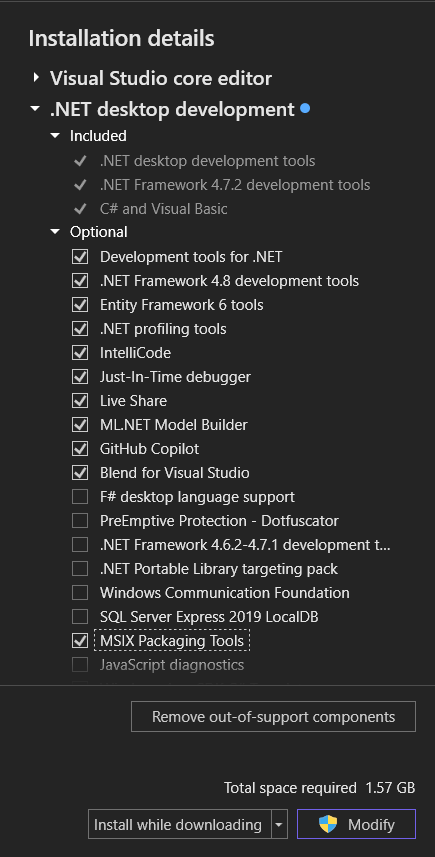
\includegraphics[width=0.30\linewidth]{1.4_1.png}
    \caption{Installing the MSIX Packaging Tools in the Visual Studio Installer.}
\end{figure}

\noindent To get Visual Studio ready for packaging, I opened the Visual Studio Installer and made sure the MSIX Packaging Tools component was checked and installed.

\begin{figure}[H]
    \centering
    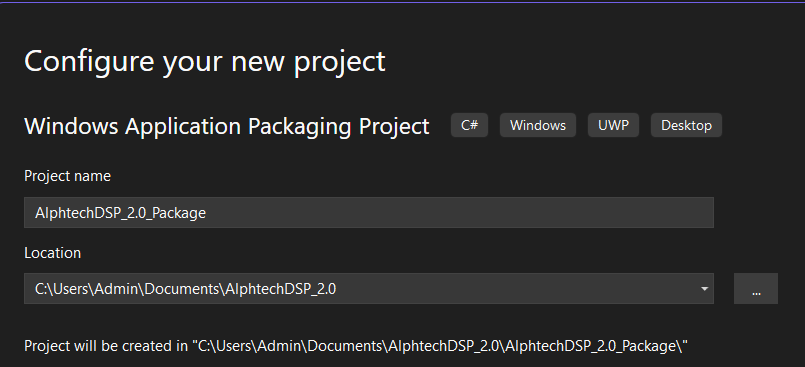
\includegraphics[width=0.58\linewidth]{1.4_2.png}
    \caption{Adding a new Windows Application Packaging Project to the solution.}
\end{figure}

\noindent Back in my solution, I added a new Windows Application Packaging Project and named it AlphtechDSP\_2.0\_Package.

\begin{figure}[H]
    \centering
    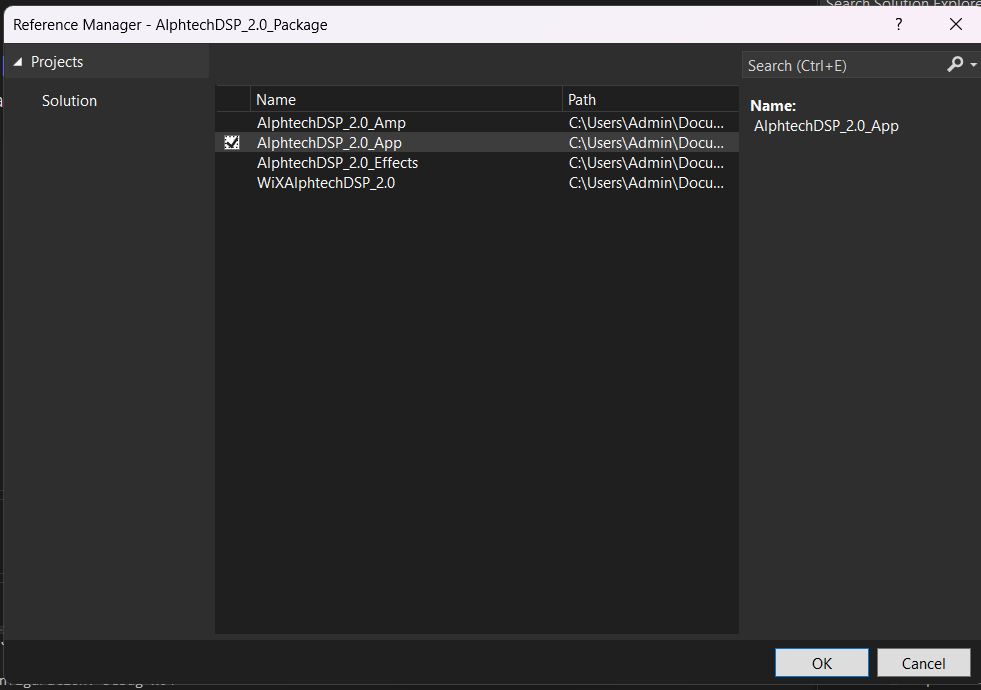
\includegraphics[width=0.60\linewidth]{1.4_3.png}
    \caption{Adding a project reference to AlphtechDSP\_2.0\_App.}
\end{figure}

\noindent I then opened the Reference Manager for the new packaging project and ticked the box for AlphtechDSP\_2.0\_App. Referencing the main application ensures that all of its project dependencies and DLL files are automatically harvested and included in the package too.

\begin{figure}[H]
    \centering
    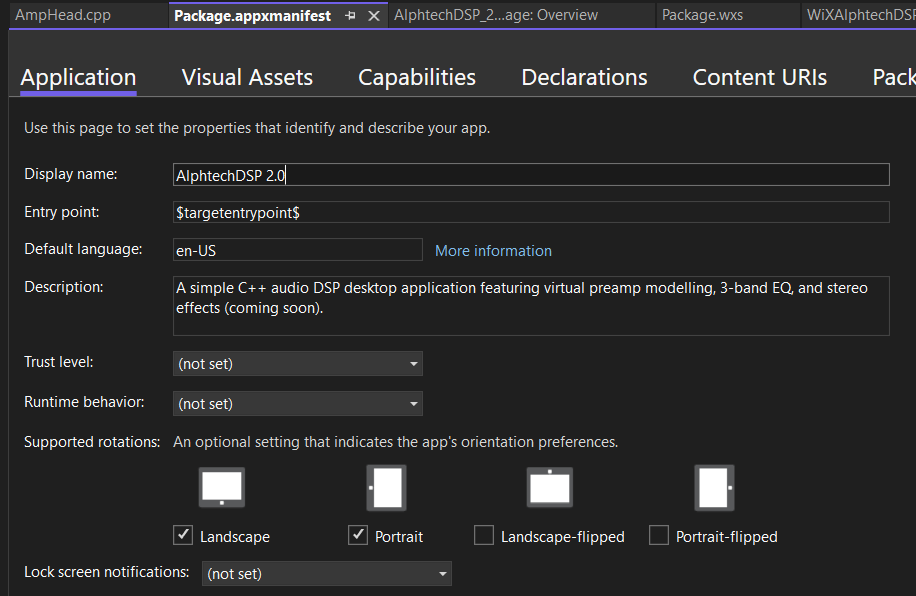
\includegraphics[width=0.60\linewidth]{1.4_4.png}
    \caption{Opening the package manifest to configure app details.}
\end{figure}

\noindent Next I opened the package manifest to set up the app details such as display name and description.

\begin{figure}[H]
    \centering
    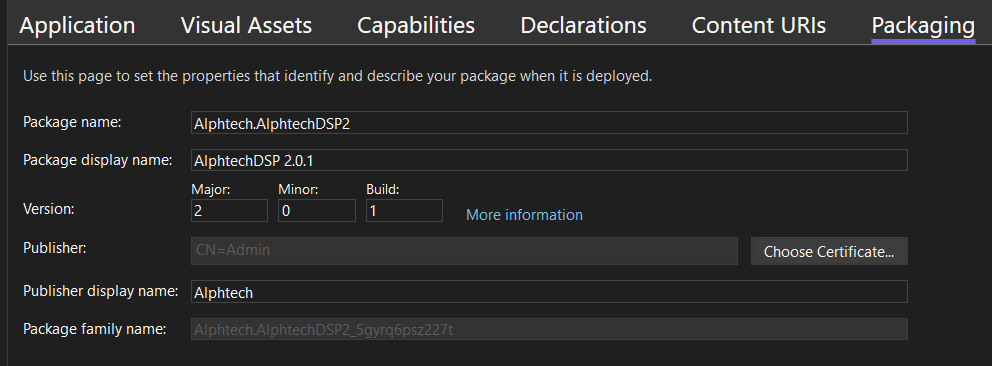
\includegraphics[width=0.60\linewidth]{1.4_5.png}
    \caption{Updating the package display name and version number in the Packaging tab.}
\end{figure}

\noindent In the Packaging tab of the manifest, I updated the package display name and set the version number to 2.0.1.0 to match the current build.

\begin{figure}[H]
    \centering
    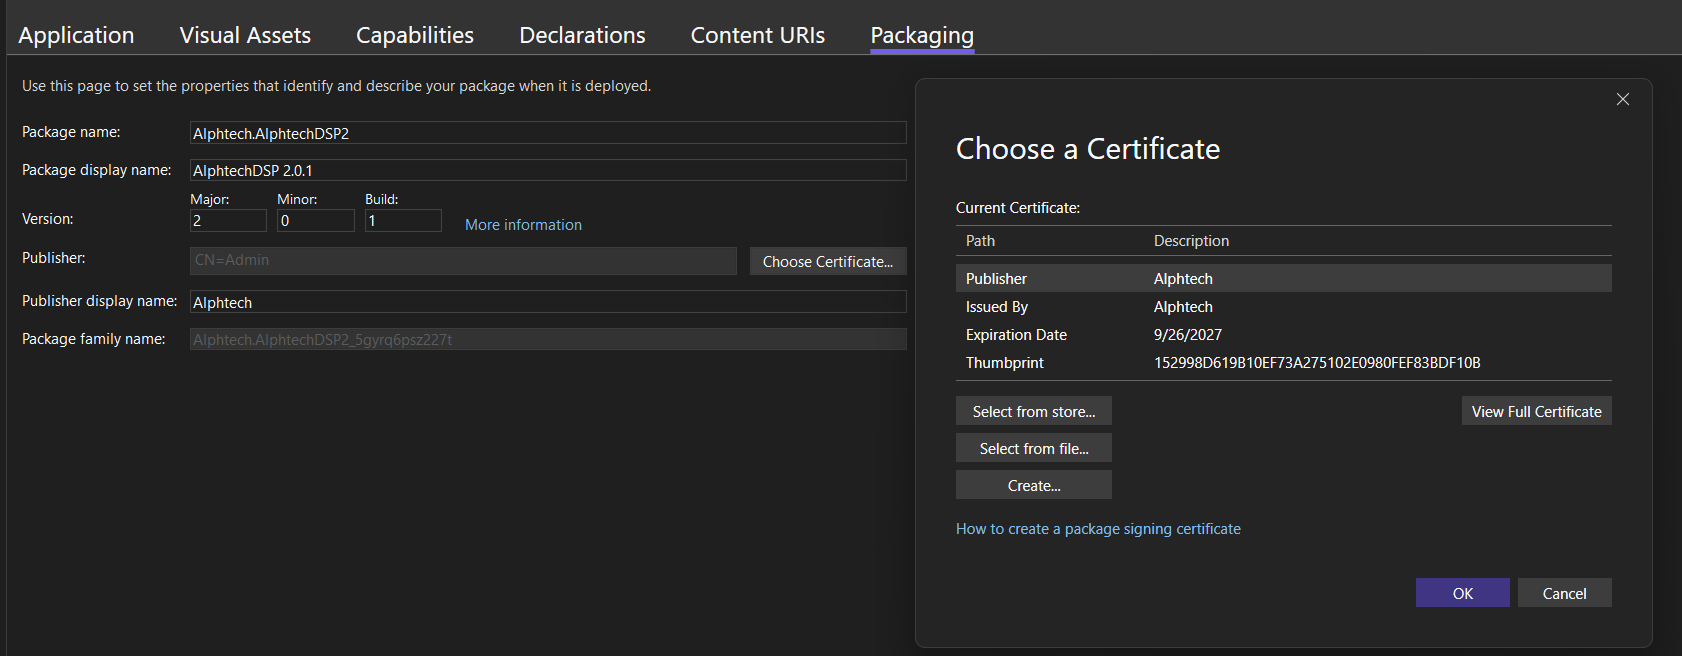
\includegraphics[width=0.60\linewidth]{1.4_6.png}
    \caption{Generating a local test certificate for package signing.}
\end{figure}

\noindent I also generated a local test certificate in the same tab so the package could be signed during the build process.

\begin{figure}[H]
    \centering
    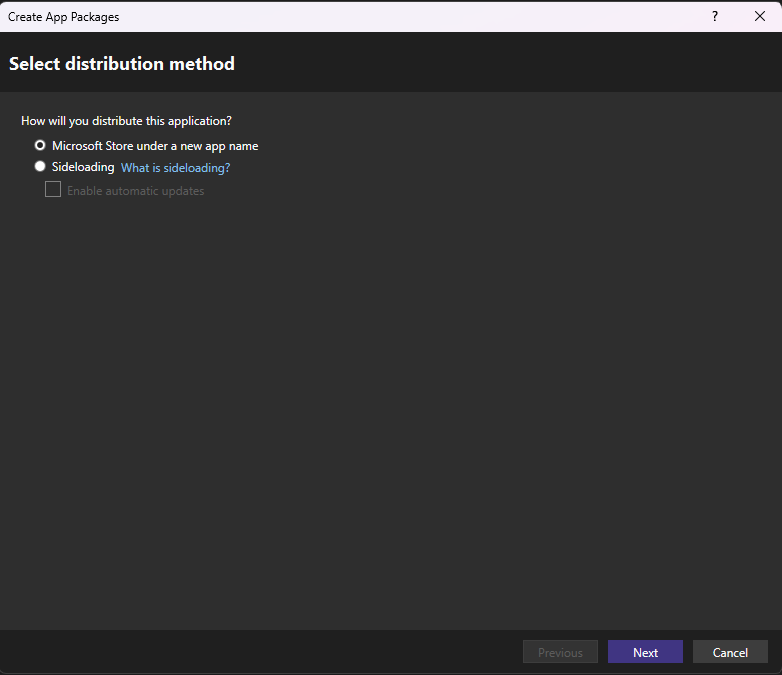
\includegraphics[width=0.60\linewidth]{1.4_7.png}
    \caption{Starting the Create App Packages wizard to distribute to the Microsoft Store.}
\end{figure}

\noindent With the configuration done, I right clicked the packaging project and started the Create App Packages wizard. I chose the option to distribute to the Microsoft Store under a new app name.

\begin{figure}[H]
    \centering
    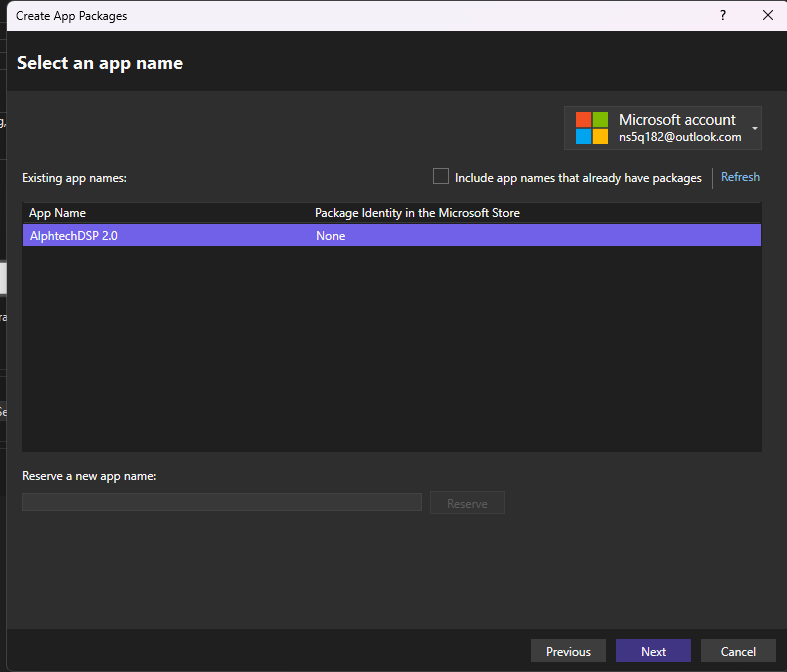
\includegraphics[width=0.60\linewidth]{1.4_8.png}
    \caption{Selecting the reserved app name after signing in with the Microsoft account.}
\end{figure}

\noindent The wizard prompted me to sign in with my Microsoft account. After logging in, it found the AlphtechDSP 2.0 name I reserved earlier and I selected it.

\begin{figure}[H]
    \centering
    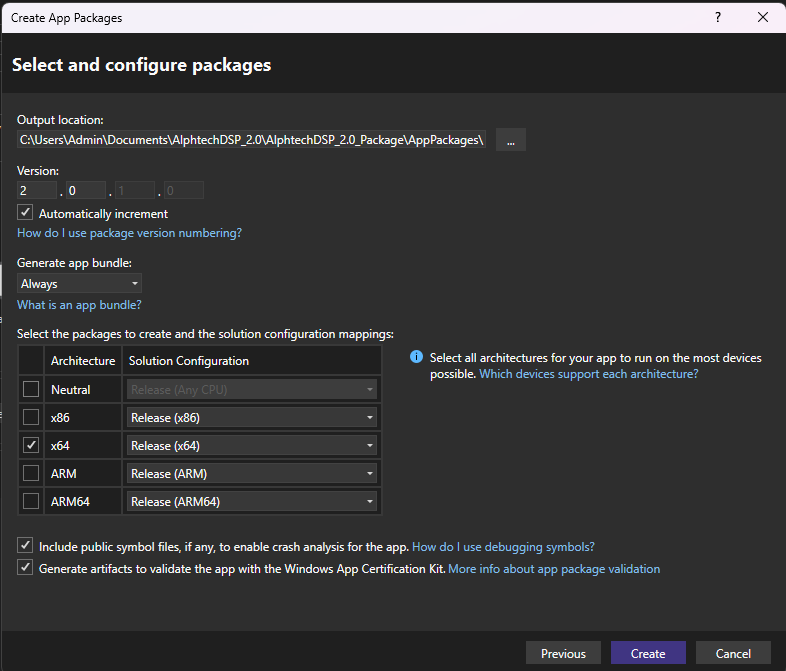
\includegraphics[width=0.60\linewidth]{1.4_9.png}
    \caption{Configuring the package architecture for x64 only.}
\end{figure}

\noindent I then configured the package architecture. I unchecked the neutral option and specifically checked x64 to ensure it builds correctly for modern processors.

\begin{figure}[H]
    \centering
    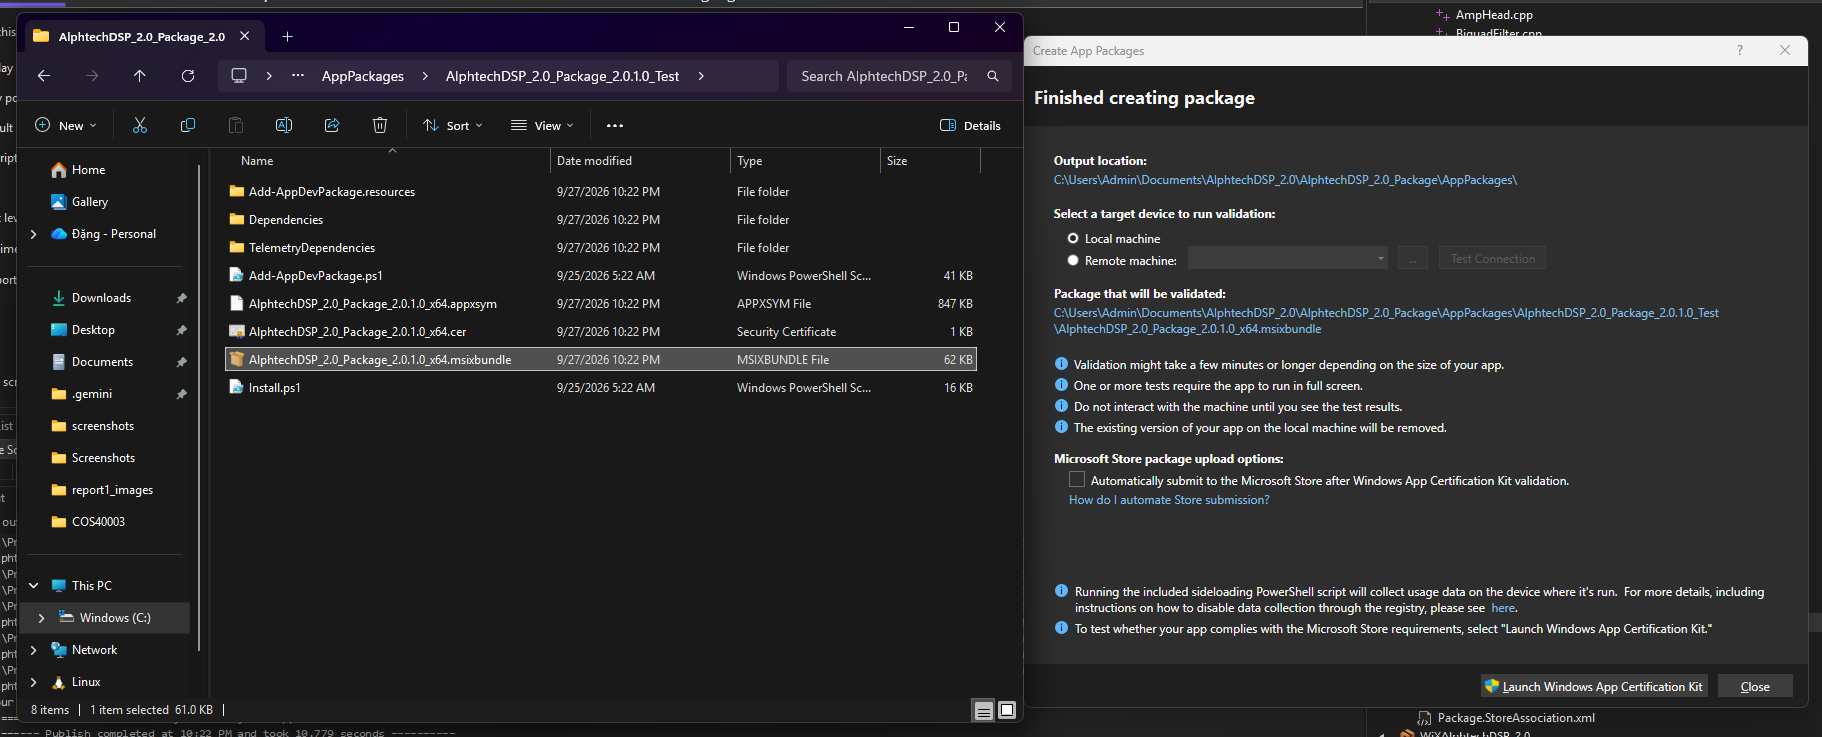
\includegraphics[width=0.60\linewidth]{1.4_10.png}
    \caption{Visual Studio completing the build of the MSIX bundle.}
\end{figure}

\noindent Visual Studio then compiled the project and built the final MSIX bundle. A confirmation window popped up and I opened the output folder to verify the generated package was there.

\begin{figure}[H]
    \centering
    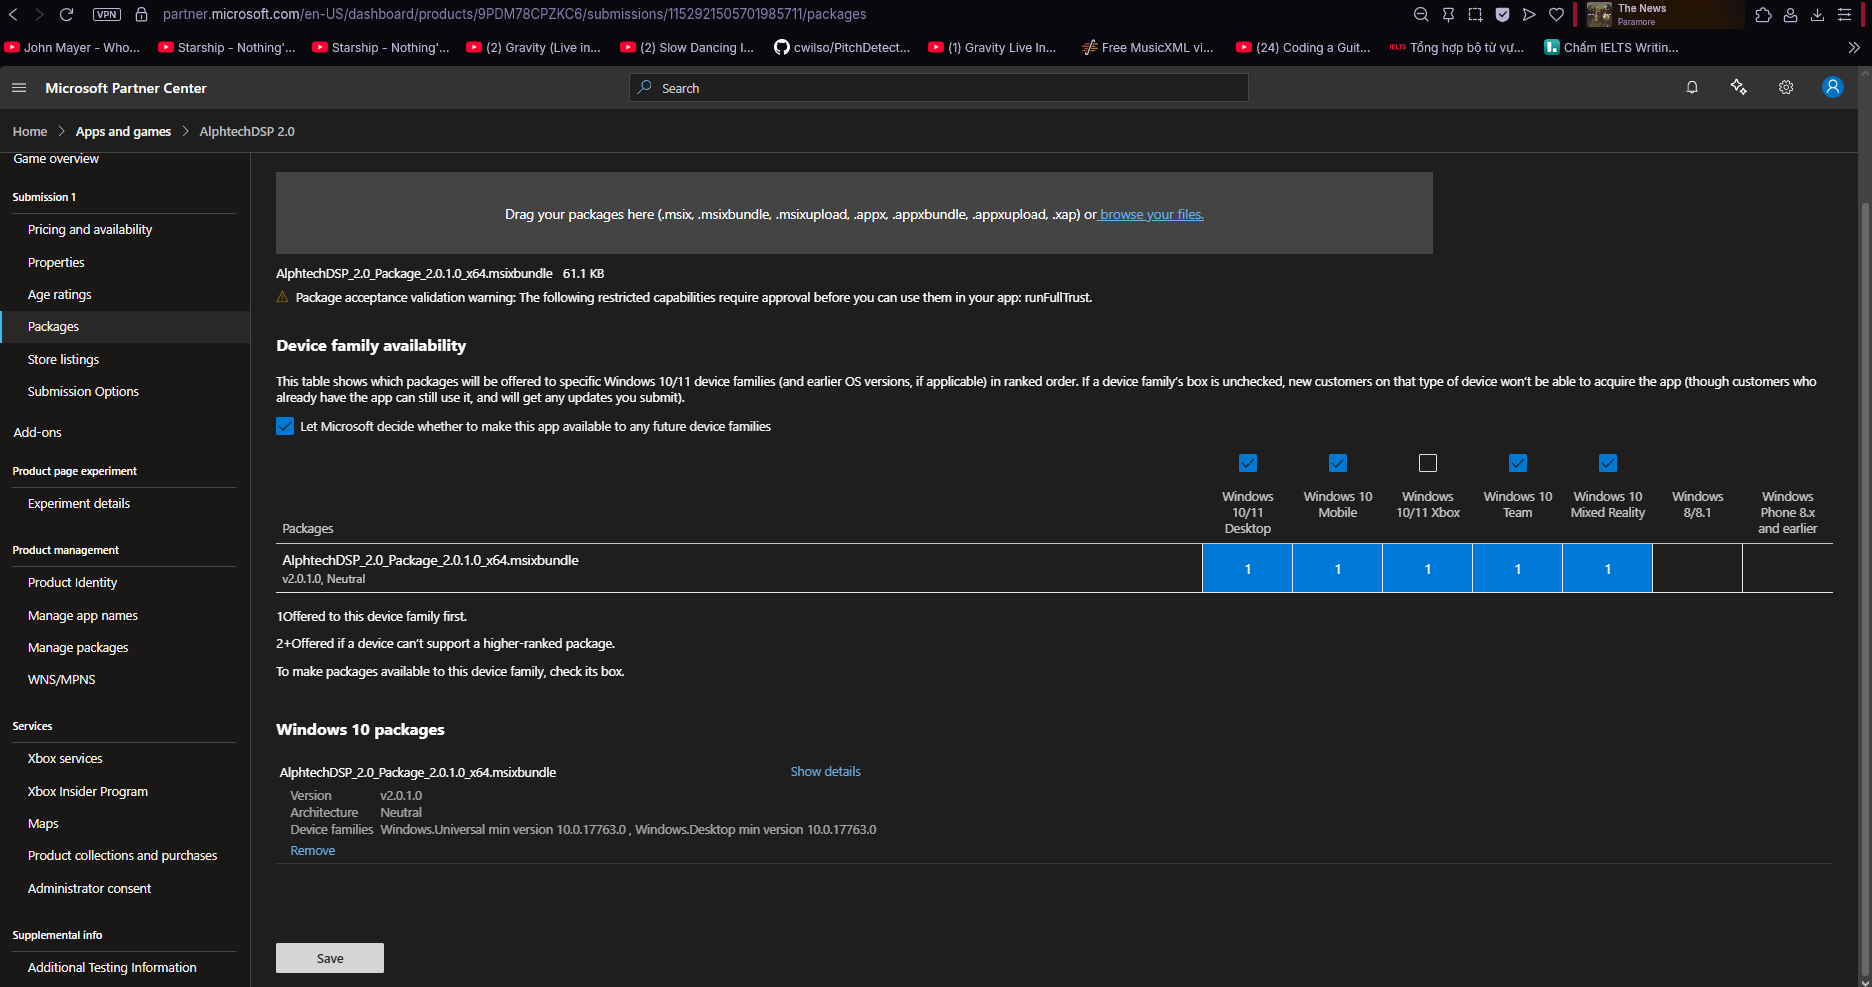
\includegraphics[width=0.60\linewidth]{1.4_11.png}
    \caption{Uploading the MSIX bundle to the for validation.}
\end{figure}

\noindent I returned to Microsoft Partner Center and uploaded the newly created MSIX bundle into the Packages section of the draft submission. After some short processing time, the package was approved.

\begin{figure}[H]
    \centering
    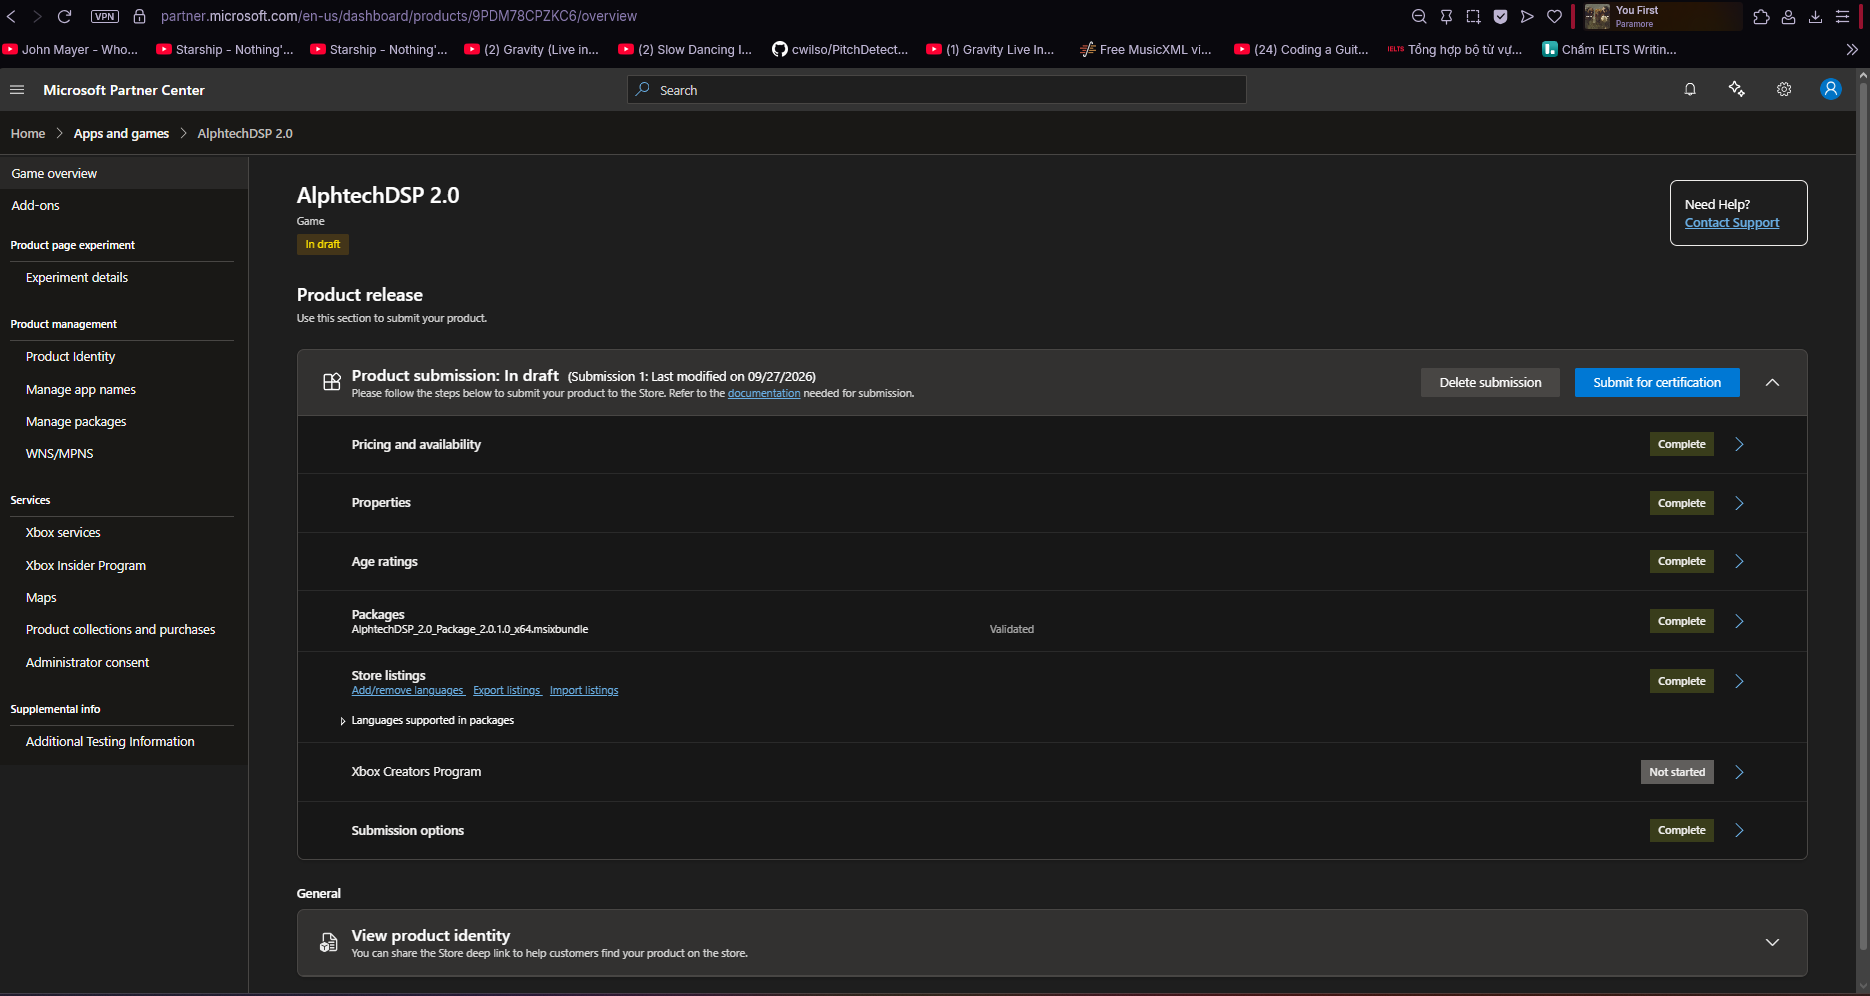
\includegraphics[width=0.60\linewidth]{1.4_13.png}
    \caption{Filling out the store listing details including pricing, properties, and description.}
\end{figure}

\noindent I then filled out the rest of the store listing detail sections. The properties were configured as follows:
\begin{itemize}
    \item \textbf{Pricing and availability:} Set to Free (0 USD).
    \item \textbf{Properties:} Categorized under the Music genre and linked the GitHub privacy policy
    (\url{https://github.com/mikedevman/AlphtechDSP-2.0/blob/master/PRIVACY.md}).
    \item \textbf{Store listings:} Added a description and a screenshot of the application.
\end{itemize}

\begin{figure}[H]
    \centering
    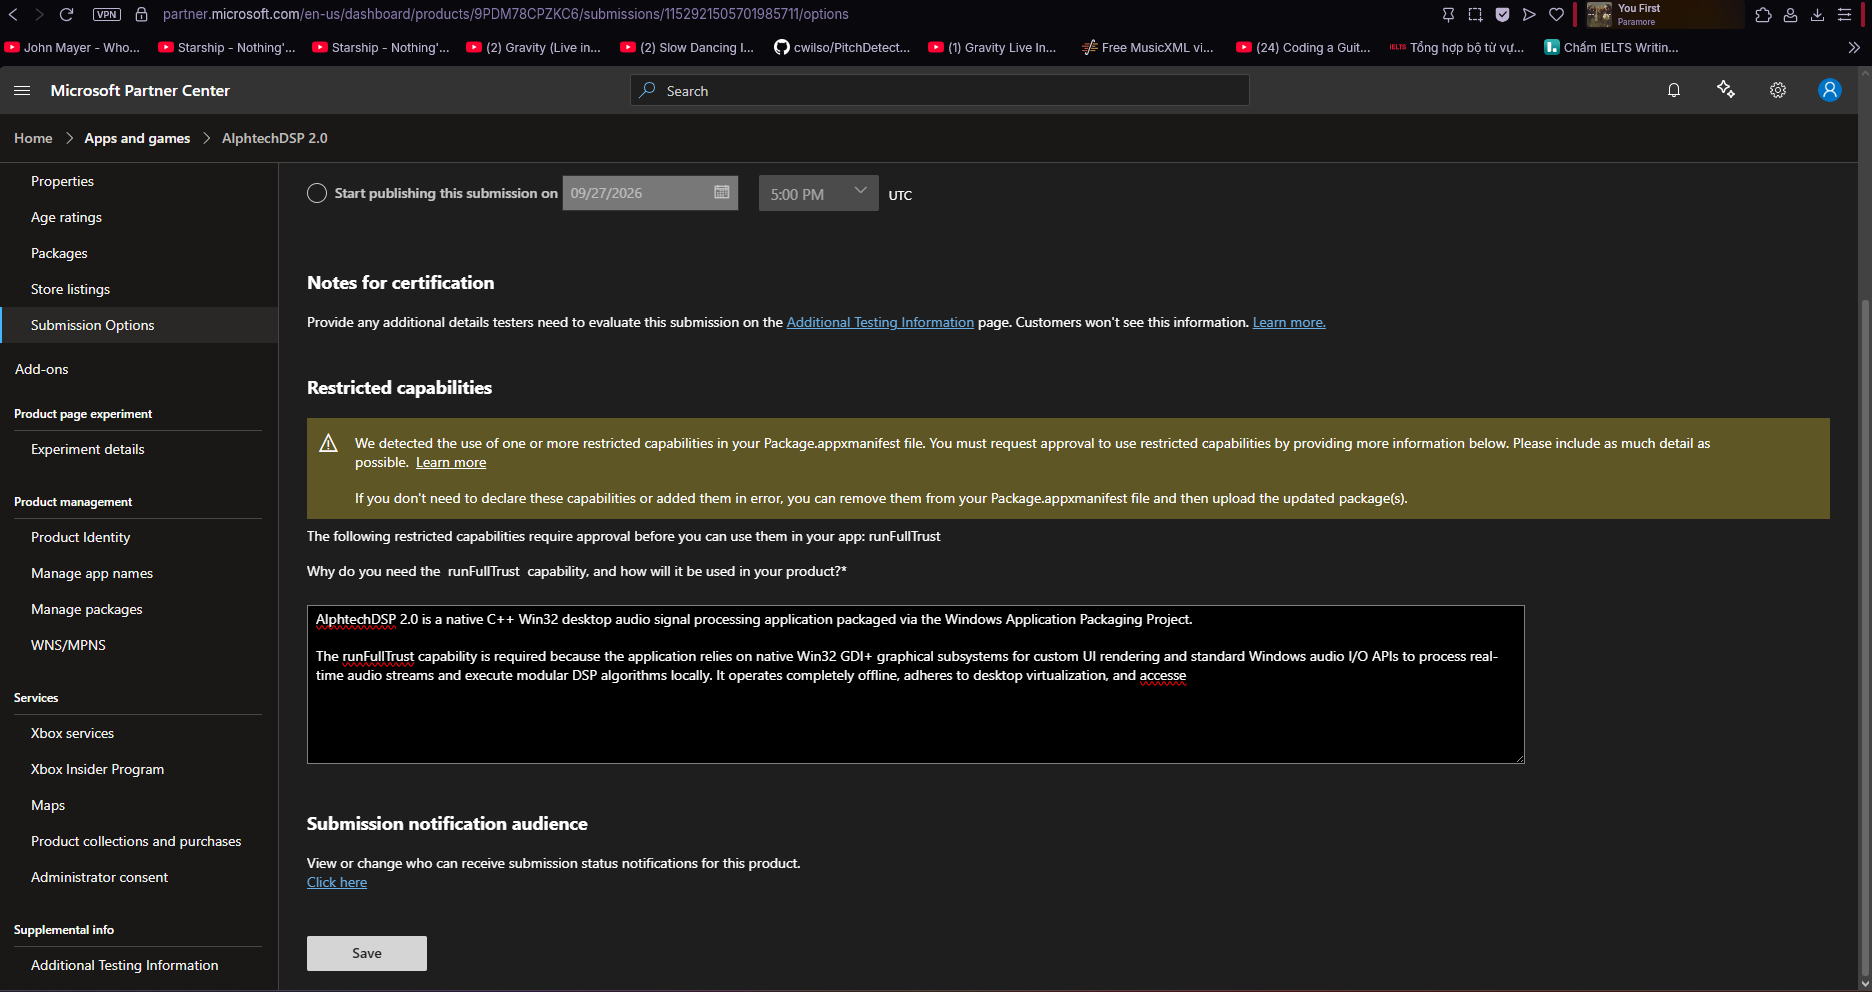
\includegraphics[width=0.60\linewidth]{1.4_12.png}
    \caption{Providing justification for the \texttt{runFullTrust} capability.}
\end{figure}

\noindent Because this is a native C++ Win32 application, it requires the \texttt{runFullTrust} capability. In the \textbf{Submission options} section, I had to provide a justification for this, explaining that it needs full trust for real-time audio processing and custom UI rendering using standard Windows APIs. Once all sections were marked complete (except for \textbf{Xbox Creators Program}, which is not needed for this application), I was ready to submit.

\begin{figure}[H]
    \centering
    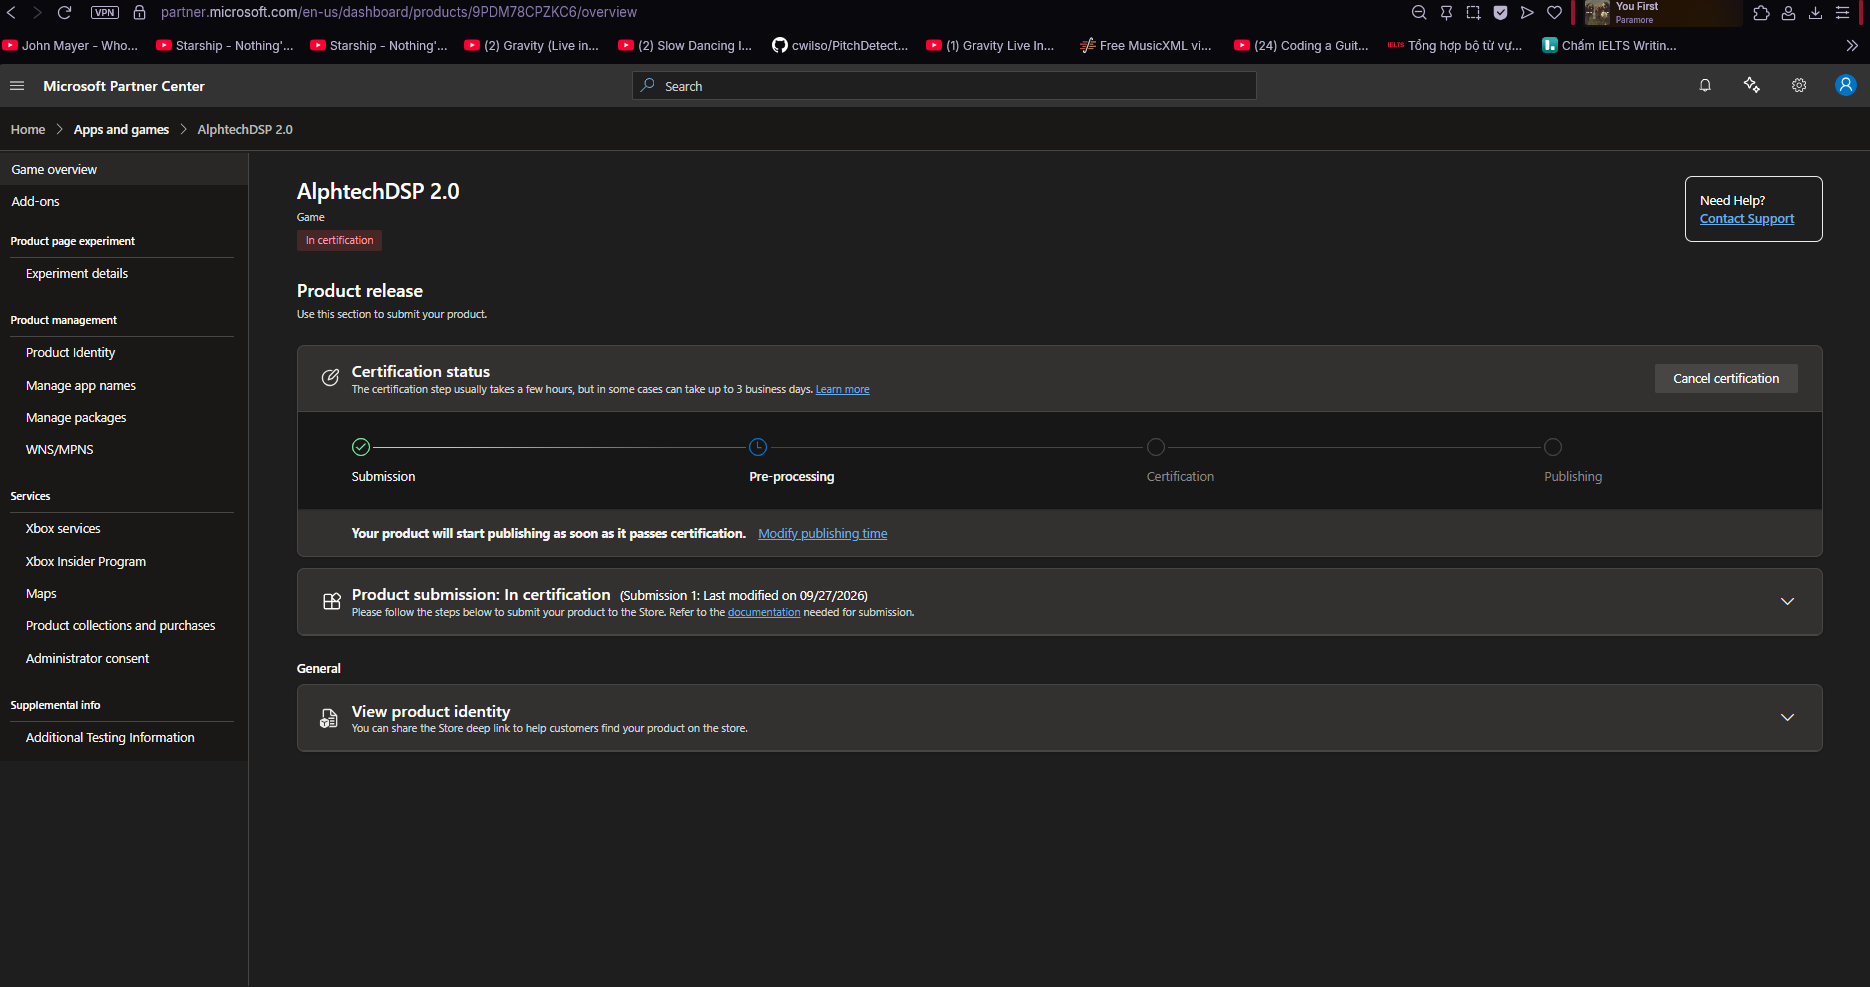
\includegraphics[width=0.60\linewidth]{1.4_14.png}
    \caption{The certification status tracker showing the submission is under processing.}
\end{figure}

\noindent Finally, I clicked the Submit for certification button. The dashboard updated to show the certification status tracker, which marked the submission step as completed, and we will need to wait for the final processing and approval.

\vspace{8pt}

\noindent At the time of submitting this report, the application is still under processing. If you want to try it out once it is published, you can search for \textbf{AlphtechDSP 2.0} directly in the Microsoft Store.

\vspace{20pt}
\begin{center}
\textbf{--- THE END ---}
\end{center}

\end{document}
